\documentclass[12pt]{article}
\usepackage{fancyhdr}
\usepackage{amsmath,amsthm,amssymb,dsfont,enumerate,color}
\usepackage[top=1in, bottom=1in]{geometry}
\usepackage{tikz}
\usepackage{tikz-3dplot}
\usetikzlibrary{patterns}
\tdplotsetmaincoords{70}{110}
\usetikzlibrary{arrows.meta}
\fancyhead[L]{MAT473}
\fancyhead[R]{Topics}
\fancyfoot[L]{Name: \underline{\hspace{2in}}}
\fancyfoot[R]{\large \thepage}
\fancyfoot[C]{this}
\newcommand{\bbA}{\mathbb{A}}
\newcommand{\bbB}{\mathbb{B}}
\newcommand{\bbC}{\mathbb{C}}
\newcommand{\End}{\operatorname{End}}
\newcommand{\Ann}{\operatorname{Ann}}
\newcommand{\bbD}{\mathbb{D}}
\newcommand{\bbE}{\mathbb{E}}
\newcommand{\bbF}{\mathbb{F}}
\newcommand{\bbG}{\mathbb{G}}
\newcommand{\bbH}{\mathbb{H}}
\newcommand{\bbI}{\mathbb{I}}
\newcommand{\bbJ}{\mathbb{J}}
\newcommand{\bbK}{\mathbb{K}}
\newcommand{\bbL}{\mathbb{L}}
\newcommand{\bbM}{\mathbb{M}}
\newcommand{\bbN}{\mathbb{N}}
\newcommand{\bbO}{\mathbb{O}}
\newcommand{\bbP}{\mathbb{P}}
\newcommand{\bbQ}{\mathbb{Q}}
\newcommand{\bbR}{\mathbb{R}}
\newcommand{\R}{\mathbb{R}}
\newcommand{\bbS}{\mathbb{S}}
\newcommand{\bbT}{\mathbb{T}}
\newcommand{\bbU}{\mathbb{U}}
\newcommand{\bbV}{\mathbb{V}}
\newcommand{\bbW}{\mathbb{W}}
\newcommand{\bbX}{\mathbb{X}}
\newcommand{\bbY}{\mathbb{Y}}
\newcommand{\bbZ}{\mathbb{Z}}
\newcommand{\bbk}{\mathbb{k}}
\newcommand{\Ab}{\mathcal{Ab}}
\newcommand{\obj}{\operatorname{obj}}
\newcommand{\mor}{\operatorname{mor}}
\newcommand{\Tor}{\operatorname{Tor}}
\newcommand{\Hom}{\operatorname{Hom}}
\newcommand{\Mat}{\operatorname{Mat}}

\newcommand{\calA}{\mathcal{A}}
\newcommand{\calB}{\mathcal{B}}
\newcommand{\calC}{\mathcal{C}}
\newcommand{\calD}{\mathcal{D}}
\newcommand{\calE}{\mathcal{E}}
\newcommand{\calF}{\mathcal{F}}
\newcommand{\calG}{\mathcal{G}}
\newcommand{\calH}{\mathcal{H}}
\newcommand{\calI}{\mathcal{I}}
\newcommand{\calJ}{\mathcal{J}}
\newcommand{\calK}{\mathcal{K}}
\newcommand{\calL}{\mathcal{L}}
\newcommand{\calM}{\mathcal{M}}
\newcommand{\calN}{\mathcal{N}}
\newcommand{\calO}{\mathcal{O}}
\newcommand{\calP}{\mathcal{P}}
\newcommand{\calQ}{\mathcal{Q}}
\newcommand{\calR}{\mathcal{R}}
\newcommand{\calS}{\mathcal{S}}
\newcommand{\calT}{\mathcal{T}}
\newcommand{\calU}{\mathcal{U}}
\newcommand{\calV}{\mathcal{V}}
\newcommand{\calW}{\mathcal{W}}
\newcommand{\calX}{\mathcal{X}}
\newcommand{\calY}{\mathcal{Y}}
\newcommand{\calZ}{\mathcal{Z}}
\newcommand{\iitem}{\vfill \item}
\newcommand{\image}{\operatorname{image}}
\newcommand{\topic}[1]{\textcolor{blue}{#1}}
\newcommand{\answerbox}{\begin{flushright}
    \begin{tikzpicture}
      \draw (0,0) rectangle (5,-1.75);
    \end{tikzpicture}\end{flushright}}
\newcommand{\solution}[1]{\textcolor{red}{#1}}
\newcommand{\points}[1]{\ [#1pts]}
%\renewcommand{\solution}[1]{}
\newcounter{excounter}[subsection]
\setcounter{excounter}{0}
\newcommand{\exercise}[1]{
\addtocounter{excounter}{1}
\textcolor{red}{\fbox{\Large \Roman{section}.\roman{subsection}.\arabic{excounter}} #1}
}
\begin{document}
\pagestyle{fancy}
\tableofcontents
\setcounter{section}{6}
\section{Basics}
\label{sec:basics}

\subsection{Introduction to rings}


\begin{description}
\item[Definition: Ring] $(R,+)$ is an abelian group, $\cdot$ is
  associative, left-and-right distributivity; can be commutative or
  not; can have identity or not (some always assume yes)
\item[Properties: Ring]\ 
  \begin{enumerate}
  \item $0a=0$ for all $a\in R$;
  \item If $1\in R$, its additive inverse is $-1$, and $-a=(-1)a$;
  \end{enumerate}
\item[Definition: division ring] A ring $R$ with unity $1\neq 0$ is a
  division ring if for each $a\in R\setminus \{0\}$, there is an
  element $b\in R$ such that $ab=ba=1$ (i.e., $R\setminus \{0\}$ is a
  group under $\cdot$). If it's commutative, $R$ is a
  field. 
\item[Examples: Rings]\ 
  \begin{enumerate}
  \item Trivial: all products are zero (can't contain identity)
  \item Zero ring
  \item Integers
  \item Rationals, reals, complex
  \item $\bbZ/n\bbZ$, but there's something to check here
  \item $\operatorname{Mat}_{n\times n}(\bbF)$
  \item Quaternion ring $\bbH = \{a+bi+cj+dk\mid a,b,c,d\in \bbR\}$
    with $ij=k$, $jk=i$, $ki=j$, and minuses if you reverse
  \item Rings of functions: $Y^X=\{f: X\rightarrow Y\}$. If $Y$ is a
    ring, then define $(f+g)(x)=f(x)+g(x)$ and
    $(fg)(x)=f(x)g(x)$. \exercise{When is it unital? When is it
      commutative?} \exercise{What if we require the functions to have
      property $F$?}
  \item Given a field $F$, $F[x_1,\dotsc, x_n]$ polynomials,
    $F(x_1,\dotsc, x_n)$ rational functions, $F[[x_1,...,x_n]]$ formal
    power series, $F[x]/(x^m)$ in which $x^m$ is set equal to zero,
    and others...
  \item Weird one... perhaps: Let $n$ be an integer, and $F$ be a
    field. Let $FQ$ denote the vector space defined on the basis
    elements $t_{ij}$ where $1\leq i \leq j \leq n$. Define
    multiplication of these elements via $t_{ij}t_{kl}=\begin{cases}
      t_{il} & \textrm{~if j=k}\\ 0 &
      \textrm{~otherwise}\end{cases}$ and extend this multiplication
    linearly. This is called the \emph{path algebra} associated to the
    directed graph $1\rightarrow 2 \rightarrow \dotsc \rightarrow n$.
  \item $R[\sqrt{d}]=\{a+b\sqrt{d} \mid a,b\in R\}$ (suppose $R$ is
    commutative) where $d$ is some integer. We make sense of
    multiplication via
    $(a+b\sqrt{d})(a'+b'\sqrt{d})=aa'+d(bb')+(ab'+ba')\sqrt{d}$ and $d
    r$ is taken to mean $\underbrace{r+r+\dotsc+r}_d$. 
  \end{enumerate}
\item[Definition: Zero divisor \& Unit] $a\in R\setminus \{0\}$ is a
  \emph{zero divisor} if $\exists b\in R$ such that $ab=0$ or
  $ba=0$. $a$ is \emph{unit} if $\exists b\in R$ such that $ab=1$. The
  set of units of $R$ is denoted $R^\times$. (Note: it is a group!)
\item[Exercise: zero divisors/units] \exercise{Prove that if $a$ is a
    unit, it is not a zero divisor, and that if $a$ is a zero divisor,
    then it is not a unit.} \exercise{Find an example of a ring $R$
    and an element $a$ where $a$ is neither a zero divisor nor a
    unit.}
\item[Exercise: units/zero divisors examples] \exercise{Describe the
    units and zero divisors of $\bbZ$.} \exercise{Describe the set of
    zero divisors of $\bbZ/n\bbZ$.} \exercise{Describe the units in
    $\bbZ/n\bbZ$.}
\item[Exercise: quadratic number field] \exercise{Show that
    $\bbQ[\sqrt{d}]$ has no zero divisors (and hence that
    $\bbZ[\sqrt{d}]$ has no zero divisors).} \exercise{Show that
    $\bbQ[\sqrt{d}]$ is a field.}
\item[Definition: integral domain] A \emph{commutative ring} with no
  zero divisors is an integral domain. 
\item[Property: cancellation in integral domains] \exercise{In an
    integral domain, $ab=0$ implies $a=0$ or $b=0$, so $ab=ac$ with
    $a\neq 0$ implies $b=c$.}
  \item[Exercise] \exercise{A finite integral domain is a field!}
  \item[Definition: subring] A subring is a subgroup that is also
    closed under multiplication. It is assumed to have the same
    identity if it has one. 
  \item[Exercises]\ 
    \begin{itemize}
    \item \exercise{The center of a ring is the set of all elements
        that commute with everything. Prove that the center is a
        subring. Prove that the center of a division ring is a field.}
    \item \exercise{Suppose that $F,G$ are two fields and $F\subset
        G$. Prove that $G$ is a vector space over $F$ (hence it makes
        sense to talk about its dimension over $F$).}
    \item \exercise{Prove that if $R$ is an integral domain, the equation $ax=b$
        has at most one solution $x$ for any pair $a,b\in R$ with $a$
        and $b$ not both equal to zero.}
    \item \exercise{Prove that if $R$ is an integral domain, there are
        at most two solutions to the equation $ax^2=b$ for any $a,b\in
        R$ with $a$ and $b$ not both equal to zero. }
      \item \exercise{Let $I$ be some indexing set, and $R_i$ be a
          ring for each $i\in I$. Define $\prod\limits_{i\in I} R_i$
          to be the direct product ring (Cartesian product with
          componentwise addition and multiplication). Prove that this
          is commutative if and only if each $R_i$ is, an integral
          domain if and only if each $R_i$ is, and a ring with unity
          if and only if each $R_i$ is.}
      \item \exercise{Consider the subset $\bigoplus\limits_{i\in I}
          R_i$ within $\prod\limits_{i\in I} R_i$ of elements
          $(r_1,r_2,\dotsc)$ in which all but finitely many of the
          $r_i$ are equal to zero. Prove that this subset is a
          ring. Explain further why this \emph{direct sum} ring does
          not have an identity if $I$ is infinite (even if each $R_i$
          does have an identity).}
      \item \exercise{Let $R$ be a commutative ring with identity, and
          $G=\{g_1,\dotsc, g_n\}$ be a finite group with operation
          written as multiplication (no matter what it really
          is). Define $RG$ to be the set of formal sums 
          \[a_1g_1+\dotsc + a_n g_n \] where $a_i\in R$ and $g_i \in
          G$. Define addition componentwise, and multiplication by
          $(ag_i)(bg_j)=(ab)(g_ig_j)$. Show that $RG$ is a ring, which
          is commutative if and only if $G$ is Abelian. }
      \item \exercise{Prove that if in the group ring $RG$, any
          element $1g_i$ is a unit, but that if $G\neq \{e\}$, there
          are always zero divisors.}
      \item \exercise{Prove that the real quaternion ring is a
          division ring.}
    \end{itemize}
\end{description}

\setcounter{subsection}{2}
\subsection{Ring homomorphisms}
\label{sec:ring-homomorphisms}

\begin{description}
\item[Definition: homomorphism/isomorphism] A ring homomorphism $\phi:
  R\rightarrow R'$ is a group homomorphism of the additive groups
  $(R,+), (R',+')$ satisfying $\phi(ab)=\phi(a)\phi(b)$ for all
  $a,b\in R$. An isomorphism is a bijective homomorphism. 
\item[Exercise: inverse homomorphism] \exercise{If $\phi: R\rightarrow
    S$ is a ring homomorphism that is bijective, then $\phi^{-1}:
    S\rightarrow R$ is also a ring homomorphism.}
\item[Definition: image and kernel] The \emph{kernel} of a ring
  homormophism is the set $\{r\in R \mid \phi(r)=0\}$. 
\item[Exercise: substructure of kernel and image] \exercise{The image
    of a ring homomorphism is a subring of the codomain.}
  \exercise{The kernel $K$ of a ring homomorphism $\phi: R\rightarrow S$
    is a subring of the domain with the additional property that $r
    k\in K$ for any $k\in K$ and $r\in R$.}
\item[Exercise: examples]\ 
  \begin{itemize}
  \item \exercise{For any positive integer $n$ define the map $\phi:
      \bbZ\rightarrow \bbZ/n\bbZ$ via $\phi(m)=[m]_n$ (the congruence
      class of $m$ modulo $n$.) Compute its kernel.}
  \item \exercise{Let $F$ be a field, and $a\in F$ be a fixed
      element. Define $\operatorname{ev}_a: F[x]\rightarrow F$ by the
      following assignment: $\operatorname{ev}_a(p(x)) = p(a)$. Prove
      that $\phi$ is a ring homomorphism. Describe the kernel.} 
  \item \exercise{Challenge: Consider the homomorphism from the
      above. Show that if $F=\bbC$, then
      $\operatorname{ker}(f)=\{p(x)\in \bbC[x] \mid p(x)=(x-a)q(x),
      \exists q(x)\in \bbC[x]\}$. }
  \item \exercise{Let $m$ be an integer. Determine the values of $m$
      for which the function $\phi_m: \bbZ\rightarrow \bbZ$ given by
      $\phi_m(n)\mapsto m\cdot n$ is a homomorphism. }
  \end{itemize}
\item[Definition: quotient rings] So the kernel $\ker \phi$ is a
  homomorphism $\phi: R\rightarrow S$ is, at core, an
  additive subgroup of the $R$. From groups, we know that it is
  normal, and the first isomorphism theorem for groups tells us that
  $R/\ker \phi$ is isomorphic (as a group) to $\image
  \phi$ via $\tilde{\phi}: r+\ker \phi\mapsto
  \phi(r)$. \exercise{Prove that $\tilde{\phi}$ is a ring
    homomorphism.}
\item[Exercise] \exercise{Let $\bbQ$ be the rational number field, and consider
  the ring $\bbQ[x]$. Define the function $\varphi: \bbQ[x]\rightarrow
  \bbR$ by $\varphi(f)=f(\sqrt{5})$.
  \begin{enumerate}
  \item Compute the kernel of $\varphi$. 
  \item Show that the image of $\varphi$ is isomorphic to
    $\bbQ[\sqrt{5}]$. 
  \end{enumerate}}
\item[Definition: ideals] Motivated by the additional structure of the
  kernel of a homomorphism, define an ideal. Let $I$ be a subgroup of
  $(R,+)$. Then $I$ is a
  \begin{itemize}
  \item \emph{left ideal} if $r x \in I$ for all pairs
    $r\in R$ and $x\in I$;
  \item \emph{right ideal} if $xr \in I$ for all pairs $r\in R$ and
    $x\in I$. 
  \item \emph{two-sided ideal} if it is both a left and right ideal. 
  \end{itemize}
we can form the quotient ring of $R$ by any two-sided ideal exactly as
we did above. 
\item[Exercise] \ Let $I\subset R$ be an ideal.
  \begin{itemize}
  \item \exercise{If there is an invertible element $x\in I$ such that
    $x^{-1}\in I$, then $I=R$. }
  \item \exercise{If $a_1,\dotsc, a_k\in I$ and $r_1,\dotsc, r_k\in
      R$ and $I$ is a left ideal, then $a_1r_1+\dotsc+a_kr_k\in I$. }
  \item \exercise{Let $I\subset \bbQ[x]$ be the set of polynomials
      whose summands are of degree at least 2. Compute the dimension
      of $\bbQ[x]/I$ as a vector space over $\bbQ$. Find a complete
      set of representatives for the elements of $\bbQ[x]/I.$}
  \item \exercise{List the ideals of $\bbZ/n\bbZ$ for each integer
      $n$. }
  \item \exercise{Prove that a commutative ring $R$ is a field if and only if it
      has no non-trivial ideals (i.e., its only ideals are $R$ and $\{0\}$.}
  \end{itemize}
\item[Exercise: examples] 
  \begin{itemize}
  \item \exercise{Describe all ideals in $\bbZ$.}
  \end{itemize}
\item[Exercise: reduction for Diophantine] The greeks (and beyond)
  were interested deeply in Diophantine equations, that is, polynomial
  equations in multiple variables with integer coefficients. The goal
  is to find all integer solutions, but this can be hard (Fermat's Last
  Theorem anyone?) Reduction modulo an integer can help because there
  are now only finitely many possibilities. \exercise{Consider the
    equation $x^2+y^2=3z^2$. Show that the only integer solution to
    this equation is the trivial one ($x=y=z=0$) by reducing modulo
    $4$ and investigating the perfect squares in this ring.}
\item[Exercise: ideal algebra] There are some nice algebraic steps
  that can be carried out with ideals. Let $I$ and $J$ be two-sided ideals:
  \begin{itemize}
  \item \exercise{Show that the sum of $I$ and $J$, defined by 
      \[I+J=\{a+b\mid a\in I,\ b\in J\}.\]}
  \item \exercise{Show that the product of $I$ and $J$, defined as the
      set of all finite sums of elements $ab$ where $a\in I$ and $b\in
      B$ is a two-sided ideal.}
\item $I^n:=I^{n-1} I$ are the powers, defined inductively. 
\item \exercise{Suppose that $\{I_j \mid j\in \Omega\}$ is a set of
    ideals in a ring $I$ (where $\Omega$ is a not-necessarily-finite
    index set). Prove that $\bigcap\limits_{j\in \Omega} I_j$ is an
    ideal.}
\item \exercise{Suppose that $I_1\subset I_2\subset \dotsc$ is a set
    of ideals in a ring $R$ that form a chain. Prove that
    $\bigcup\limits_{n=1}^\infty I_n$ is an ideal. }
  \end{itemize}
\item[Exercise: more ideal algebra] Suppose that $m,n\in \bbZ$ and
  consider the ideals $m\bbZ$ and $n\bbZ$ in $\bbZ$. \exercise{Express
    the ideal $m\bbZ+n\bbZ$ as an ideal of the form $d\bbZ$. I.e.,
    what is $d$ and why?} \exercise{Express the ideal $(m\bbZ)(n\bbZ)$
    as an ideal of the form $d\bbZ$.}
\item[Exercise: the isomorphism theorems] \ Throughout, $R$ is a ring
  with identity.
  \begin{enumerate}
  \item \exercise{Suppose that $A$ is a subring of $R$ and $I$ is an
      ideal of $R$. The set $A+I$ is defined to be the set $\{a+y\mid
      a\in A,\ y\in I\}$. Prove that 
      \[(A+I)/I \cong A/(A\cap I).\]}
  \item \exercise{Suppose that $I\subset J \subset R$ is a chain of
      ideals in $R$. Prove that $(R/I)/(J/I) \cong R/J$. }
  \item \exercise{Prove that there is a bijection between the set of
      ideals in $R$ containing $I$ and ideals in $R/I$. }
  \end{enumerate}
\end{description}

\subsection{Properties of ideals}
\label{sec:properties-ideals}

\begin{description}
\item[Definitions] Let $A$ be a subset of a ring $R$, a ring with identity.
  \begin{enumerate}
  \item We denote by $(A)$ the smallest ideal of $R$ containing
    $A$, called the \emph{ideal generated by $A$}. [Note: this is the
    intersection of all ideals that contain $A$, so by above
    exercises, it is clearly an ideal.]
  \item We have the following:
    \begin{align*}
      RA &= \{r_1a_1+\dotsc + r_n a_n \mid r_i\in R,\ a_i\in A\}\\
      AR &= \{a_1r_1+\dotsc + a_n r_n\mid r_i\in R,\ a_i\in A\}\\
      RAR&= \{r_1a_1r_1'+\dotsc + r_na_nr_n' \mid r_i, r_i'\in R,\
           a_i\in A\}.
    \end{align*}
  \item An ideal that can be generated by a single element is a
    \emph{principal ideal};
  \item An ideal that can be generated by a finite set of elements is
    called \emph{finitely generated}. 
  \end{enumerate}
\item[Exercises] \ 
  \begin{enumerate}
  \item \exercise{Prove that every ideal in $\bbZ$ is a principal
      ideal.$\star$}
  \item \exercise{Show that the ideal $(2,x)\subset \bbZ[x]$ is
      \emph{not} a principal ideal.}
  \item \exercise{Suppose that $R$ is a ring with identity and $I$ is
      a two-sided ideal in
      $R$. Prove that $I=R$ if and only if $I$ contains an invertible
      element. }
    \item \exercise{Suppose that $R$ is a commutative ring. Prove
    that $R$ is a field if and only if its only ideals are $R$ and
    $0$. As a corollary, prove that if $F$ is a field and $\varphi:
    F\rightarrow R'$ is a non-zero ring homomorphism, then $\varphi$
    is injective.}
\item \exercise{Suppose that $I$ is a two-sided ideal in the matrix ring
    $M_n(\bbC)$.} 
  \end{enumerate}
\item[Remark] If we're thinking about substructures within algebraic structures, it
often makes sense to ask about the smallest among them and the
largest. Of course, the smallest ideal in a ring $R$ is $\{0\}$, and
the largest is $R$. But perhaps we'd want to avoid those. It turns out
that the large non-trivial ones are really interesting (but you're free to think
about what the smallest might look like). 
\item[Definition: maximal] A two-sided ideal $\frak{m}\subsetneq R$ is called
  \emph{maximal} if there are no ideals $I$ with $\frak{m}\subsetneq I
  \subsetneq R$. 
\item[Exercise: Using Zorn's Lemma] \exercise{Prove that every ring
    $R$ with identity $1\neq 0$ has at least one maximal ideal. The
    proof of existence of some maximal element is often achieved using
    Zorn's lemma, which you can find in the Appendix in Dummit and
    Foote.}
\item[Exercises] \ 
  \begin{enumerate}
  \item \exercise{Suppose that $R$ is a commutative ring with
      identity. Prove that an ideal $\frak{m}\subsetneq R$ is a
      maximal ideal if and only if $R/\frak{m}$ is a field. }
This exercise is vitally important for the study of Fields and Galois
Theory. It says that if you can construct a commutative ring, $R$ and
a maximal ideal $\frak{m}$ within, then $R/\frak{m}$ is a field. As an
example, see the next exercise. 
\item \exercise{Consider the ring $\bbR[x]$. Prove that the ideal
    $(x^2+1)$ is a maximal ideal, then show that $\bbR[x]/(x^2+1)$ is
    isomorphic to a field that you're very familiar with.}
\item \exercise{Prove that $\bbZ/p\bbZ$ is a field if and only if $p$
    is a prime number.}
  \end{enumerate}
\item[Remark] Now let's think about generalizing some behavior within
  the integers. A positive integer $p>1$ is \emph{prime} if $ab=p$ implies
  $a=\pm 1$
  or $b=\pm 1$. But the really nice property is that if $ab$ is a
  multiple of $p$, then $p\mid a$ or $p mid b$.  When we cast that into the ideal corresponding to $p$, $(p)$,
  that means that if $ab\in (p)$, then $a\in (p)$ or $b\in (p)$. This
  inspires the following. 
\item[Definition: Primeness] Let $R$ be a commutative ring. An ideal
  $P\neq R$ is called \emph{prime} if $ab\in P$ implies that $a\in P$
  or $b\in P$. 
\item[Exercises] \ 
  \begin{enumerate}
  \item \exercise{Let $R=\bbQ[x,y]$. Prove that the set of polynomials
      in $R$ with 0 constant term is maximal, the ideal of all
      multiples of $x$ is prime but not maximal, and the ideal of all
      multiples of $xy$ is not prime and not maximal. }
  \item \exercise{Suppose that $R$ is a commutative ring. Prove that
      an ideal $P\subset R$ is prime if and only if $R/P$ is an
      integral domain. As a corollary, show that all maximal ideals
      are prime ideals.}
  \item \exercise{Prove that $(2,x)$ is a maximal ideal in $\bbZ[x]$.}
  \item \exercise{Let's write $F_2=\bbZ/2\bbZ$, the field with two
      elements. Consider the ideal $I$ in $F_2[x]$ generated by
      $(x^2+x+1)$. Prove that $I$ is a maximal ideal, and determine
      the addition and multiplication table for the field
      $F_2[x]/(x^2+x+1)$. Congratulations! You've witnessed a field
      with $4$ elements.}
  \end{enumerate}
\item[Concluding Remarks] What is happening here? First, recall that
  we might start by being interested in integral solutions to
  equations of the form $p(x_1,x_2,\dotsc, x_n)=0$. For example,
  $x^2+y^2-3z^2=0$. We witnessed a while back that if we were to
  reduce the coefficient set modulo 4 (i.e., reduce the polynomial via
  the ideal generated by 4) it could help us understand or restrict
  the possibilities. Think about the following progression:
  \begin{enumerate}
  \item When we only had the natural numbers, we had no solutions to
    the equations of the form $x+a=b$ when $b<a$. How frustrating! So
    let's introduce the integers. We now have additive inverses
    \emph{and} multiplication. 
  \item We notice that we have this nice property that if $a\neq 0$,
    then $ax=ay$ if and only if $x=y$. So cancellation works.
  \item But we also notice we don't \emph{always} have solutions to
    equations of the form $ax=b$, though when we do, we only have
    one. Why is that... and how could we break it? So let's introduce
    division. Now we have the rational numbers.
  \item Over the rationals, we can solve all equations of the form
    $ax=b$ when $a\neq 0$. Great!
  \item What about polynomials? A polynomial of degree $d$ with
    rational coefficients doesn't always have all of its roots
    rational, but in general there are at least $d$ of these roots
    (counting multiplicity). Cool. What do we have to do to get the
    rest of these roots? It turns out going to the reals isn't enough,
    so we actually have to pass to the complex numbers. That leap is
    two steps. The first is using analysis to pass to the real
    numbers, then using ring theory to pass to the complex numbers.
  \end{enumerate}

\end{description}

\subsection{Rings of fractions: localization}
\label{sec:rings-fractions}

Let's focus on the step from the integers to the rational numbers. The
idea is that the integers weren't robust enough to have solutions to
all equations of the form $ax=b$ where $a,b\in \bbZ$ and $a$ is
non-zero (if $a=0$, then $b$ must be zero to admit any solutions, and
we don't have a problem with that). So
we introduce inverses.
\begin{description}
\item[Remark] Fractions in the realm of integers goes like this: we
  consider the set of ordered pairs $(a,b)$ where $b\neq 0$. The first
  component is the numerator, and the second component is the
  denominator. Now we want to declare $(a,b)$ to be equivalent to
  $(c,d)$ when $ax=b$ has the same solution as $cx=d$. This would
  imply that $axd=cxb$, or $(ad-bc)x=0$. If we assume $R$ is an
  integral domain, then this means $x=0$ or $ad-bc=0$. I.e.,
  $ad=bc$. Look familiar? So we have a set of ordered pairs $\{(a,b)
  \mid a,b\in R,\ b\neq 0\}$ and an equivalence relation $(a,b)\sim
  (c,d)$ if $ad=bc$. Can we define arithmetic? 
\item[Theorem: Inversion] Suppose that $R$ is a commutative ring with identity and
  that $D\subset R$ is a \emph{multiplicative set}. I.e., if $a,b\in
  D$, then $ab\in D$, and furthermore $1\in D$. There is a ring
  $D^{-1}R$ with the following properties:
  \begin{itemize}
  \item There exists a homomorphism $\phi: R\rightarrow D^{-1}R$;
  \item If $d\in D$, then $\phi(d)$ is a unit in $D^{-1}R$;
  \item If there is any other ring $T$ and ring homomorphism $f:
    R\rightarrow T$ such that $f(d)\in T^*$ for all $d\in D$, then
    there exists a unique ring homomorphism $\tilde{f}:D^{-1}R\rightarrow T$
    such that $\tilde{f}\circ \phi = f$. 
  \end{itemize}
$D^{-1}R$ is referred to as the \emph{localization} of $R$ with
respect to $D$, or the ring of fractions of $D$ in $R$. 
\item[Exercises]\ 
  \begin{enumerate}
  \item \exercise{Consider the set $R\times D$ of ordered pairs and define a
    relation $\sim_D$ via $(r_1,d_1)\sim (r_2,d_2)$ if there exists an
    element $t\in D$ such that $t(r_1d_2-r_2d_1)=0$. Show that
    $\sim_D$ is an equivalence relation on $R\times D$.}
  \item \exercise{We define addition and multiplication on $R\times D$ in the
    way that we do on fractions:
    \begin{align*}
      (r_1,d_1)\cdot (r_2,d_2)&=(r_1r_2,d_1d_2)\\
      (r_1,d_1)+(r_2,d_2) &= (r_1d_2+r_2d_1,d_1d_2)
    \end{align*}
Prove that these operations are well-defined on $R\times D/\sim_D$. }
\item \exercise{Show that $R\times D/\sim_D$ is a ring with identity $(d,d)$ for
  any $d\in D$. (If we hadn't assumed that $R$ was a ring with
  identity, but had that $D$ was non-empty, this would give us an
  identity in $D^{-1}R$.)}
\item \exercise{Prove that the map $\phi: R\rightarrow D^{-1}R$ defined by
  $\phi(r)=(r,1)$ is a ring homomorphism and that $\phi(d)$ is a unit
  in $D^{-1}R$. }
\item \exercise{Prove that the above map is one-to-one if and only if $D$
  contains no zero-divisors. In particular, if $R$ is an integral
  domain and $0\not\in D$, this is always the case.}
\item \exercise{Lemma: Prove that if $f: R\rightarrow T$ is a ring
    homomorphism and that $f(1_R)\neq 1_T$ then
    $\operatorname{image}(f)\subset \operatorname{ZD}(T)$. In
    particular, $f(r)\not\in T^*$ for all $a\in R$.}
\item \exercise{Lemma: Prove that if $f: R\rightarrow T$ is a ring
    homomorphism with $f(1_R)=1_T$ and $d\in R^*$ then
    $f(d^{-1})=f(d)^{-1}$ (in particular, $f(d)$ is invertible).}
\item \exercise{Prove the universal property of $D^{-1}R$: If $T$ is
    any ring and $f: R\rightarrow T$ is a ring homomorphism such that
    $f(d)\in T^*$ for all $d\in D$, then there exists a unique ring
    homomorphism $\tilde{f}: D^{-1}R\rightarrow T$ such that
    $\tilde{f}\circ \phi = f$. }
  \end{enumerate}
\item[Remark] The word \emph{universal property} showed up above, and
  it might seem strange. This starts a light conversation about
  categories. Much more is to be said, but a universal property gives
  us a way to define the type of behaviour we want to see (like
  invertibility of the elements of $D$) and determine if there is a
  unique way to define this structure. 
\item[Remark] If $R$ is a field and $0\notin D$, then $D^{-1}R\cong
  R$. If $R$ is an integral domain and $D=R\setminus \{0\}$, then
  $D^{-1}R$ is a field... and this is what we wanted in the first
  place.
\item[Exercise] \exercise{Consider $\bbZ$ and the two subsets $D=2\bbZ$ and $S=\{2^n
  \mid n\in \bbZ_{\geq 0}\}$. Describe $D^{-1}\bbZ$ and
  $S^{-1}\bbZ$. Are they isomorphic? }
\item[Exercise] \exercise{If $d\in R$ is not zero and not a zero-divisor, then
  define $d^{\bbZ}=\{1,d,d^2,\dotsc,\}$. Then $(d^\bbZ)^{-1}R$ is like
  the ring of polynomials in the variable $1/d$, which we write
  $R[1/d]$. (There's something to prove here: that the powers are
  really independent.)}
\item[Exercise] \exercise{If $R$ is an integral domain and $F$ is a field
  containing $R$, then $F$ contains $\calQ R$ is isomorphic to a
  subfield of $F$. }
\item[Exercise] \exercise{Let $R$ be an integral domain and $D$ be a
  multiplicative set. Then there is a bijection between prime ideals
  in $D^{-1}R$ and prime ideals in $R$ not intersecting $D$. }
\item[Exercise] \exercise{A commutative ring is called \emph{local} if it has a
  unique maximal ideal $\mathfrak{m}$. Prove that $R-\mathfrak{m}=R^*$
  if $R$ is a local ring. }
\item[Exercise] \exercise{Consider the commutative ring with identity
    $R$ and a multiplicative set $S$. Prove that the localization
    $\varphi$ furnishes a bijection between the set of prime ideals in
    $R$ not intersecting $S$ and the prime ideals in $S^{-1}R$. }
\item[Exercise] \exercise{Let $p$ be a prime integer, and consider $S$
    the multiplicative set of integers that are \emph{not} multiples
    of $p$. (Note, this is precisely the complement of $(p)$ in
    $\bbZ$.) The localization $S^{-1}\bbZ$ is often denoted
    $\bbZ_{(p)}$. Prove that $\bbZ_{(p)}$ is a local ring with maximal
    ideal $\{\frac{t}{q} \mid t\in (p), q\in S\}$. (You may refer to
    the previous exercise.)}
\end{description}

\subsection{Interlude: Categories}
\label{sec:interl-categ-1}


A \emph{category} $\calC$ is a pair with a class of objects,
$\obj(\calC)$ and a set $\mor_\calC(A,B)$ for all pairs of objects
$A,B$ in $\calC$ such that for each triple of objects $A,B,C\in
\obj(\calC)$, there is a function $\circ: \mor_{\calC}(B,C)\times
\mor_\calC(A,B)\rightarrow \mor_\calC(A,C)$ known as
\emph{composition} that is associative on 4-tuples of objects. We
further insist that for every object $X\in \calC$, there is an element
$1_X \in \mor_\calC(X,X)$ such that $1_X\circ f = f$ and $g\circ
1_X=g$ for all $f\in \mor_\calC(Y,X)$ and $g\in \mor_\calC(X,Z)$. 

\begin{description}
\item[Examples]\
  \begin{enumerate}
  \item Let $\calC$ be the category whose objects are the positive
    integers, with $\mor_\calC (m,n)=\begin{cases} \{n/m\} & \textrm{if
        divisible}\\ \emptyset & \textrm{otherwise}\end{cases}$. So
    the \emph{morphism} set from $m$ to $n$ is either a singleton if
    $m$ doesn't divide $n$, and empty otherwise. We also need to
    furnish a \emph{composition} of functions! What should $\circ:
    \mor_\calC(m,n) \times \mor_\calC(l,m)\rightarrow \mor_\calC(l,n)$
    do? Let's assume that there \emph{is} a divisibility, that $l \mid
    m$ and $m\mid n$. Then $l\mid n$ and its morphism is $n/l$ which
    is equal to $n/m \cdot m/l$. So let's say:
    \begin{align*}
      (n/m) \circ (m/l) &= n/l
    \end{align*}
but if either set is empty, then the codomain is empty, so composition
is just the trivial map from empty set to empty set. 

This category already has an interesting object: an \emph{initial}
object, an object $\chi$ with the property that
$\mor_\calC(\chi,n)\neq \emptyset$ for all $n\in \obj(\calC)$. What is
it? Is it unique? Why? Does it have a \emph{dual} notion?
\item Let $\Ab$ be the category whose objects are finite abelian
  groups, and whose morphism sets are the set of group
  homomorphisms, with composition being... composition. Notice that the kernel of such a homomorphism is
  still a finite abelian group and the cokernel is also. This is
  called an \emph{abelian} category. 
\item Let $\mathcal{S}et$ be the category whose objects are sets and whose
  morphisms are set functions. Composition is just composition. What
  is the \emph{initial} object here? Can you realize intersection as
  an object with a universal property? What about union?
\item Vector spaces over a given field, with linear transformations. 
\item Topological spaces with continuous maps.
\item Products are universal objects, that may or may not exist:
  \fbox{Definition:} Let $I$ be an indexing set, and let $R_i$ be an
  object for each index $i\in I$. A \emph{product} of $R_i$, denoted
  $\prod\limits_{i\in I} R_i$ is an object with a morphism $p_j:
  \prod\limits_{i\in I} R_i \rightarrow R_j$ for each $j\in I$
  satisfying the following universal property: if $T$ is any other
  object in $\calC$ with morphisms $\varphi_j: T\rightarrow R_j$ for
  each $j\in J$, then there is a unique map $\Phi: \prod\limits_{i\in
    I} R_i\rightarrow T$ such that $\varphi_j \circ \Phi = p_j$ for
  each $j\in J$. 
\item You can check that the product of rings is such a universal
  object. 
\item 
  \end{enumerate}

\end{description}


\subsection{Chinese remainder theorem}
\label{sec:chin-rema-theor}

The defining structure of rings comes partly from the ring of
integers, so let's spend a little bit of time on them. We've already
seen that every ideal in $\bbZ$ is principal. In particular, every
quotient of $\bbZ$ is of the form $\bbZ/n\bbZ$. But does this
\emph{decompose} further? 
\begin{description}
\item[Definition] Ideals $A$ and $B$ in a ring $R$ are called
  \emph{comaximal} if $A+B=R$. 
\item[Theorem: Chinese Remainder Theorem] Let $A_1,\dotsc, A_k$ be
  ideals in a commutative ring $R$ with identity. Then the map
  \begin{align*}
    R& \rightarrow R/A_1 \times R/A_2 \times \dotsc \times R/A_k\\
    r &\mapsto (r+A_1,r+A_2,\dotsc, r+A_k)
  \end{align*}
is a ring homomorphism with kernel $A_1\cap A_2 \cap \dotsc \cap
A_i$. If for each pair $i,j$ with $i\neq j$ we hav $A_i$ and $A_j$ are
comaximal, then the map is surjective, and the kernel is $A_1A_2\cdots
A_k$. Thus, \[R/(A_1A_2\cdots A_k) = R/(A_1\cap A_2\cap \dotsc \cap
  A_k) \cong R/A_1 \times \dotsc \times R/A_k.\]
\item[Note] Note that if $A_i$ are principal ideals generated by
  $a_i$, then $A_1A_2\cdots A_k=(a_1a_2\cdots a_k)$. 
\item[Proof] Let's work with $k=2$. Consider $\varphi: R\rightarrow
  R/A \times R/B$ with $\varphi(r) = (r+A,r+B)$. Ring homomorphism is
  easy, the kernel is those elements with $\varphi(r)=(0+A,0+B)$ which
  means $r\in A$ and $r\in B$, so the intersection. Assuming $A$ and
  $B$ are comaximal, this means $1=a+b$ for some $a\in A$ and $b\in
  B$. But then $\varphi(r_1a+r_2b)=(r_1a+r_2(1-a) + A,
  r_1(1-b)+r_2b+B)$, which is $(r_2+A,r_1+B)$, so $\varphi$ is
  onto. Clearly $AB\subset A\cap B$ by the absorption property. Now
  suppose that $x\in A\cap B$. Then $x=x(a+b)=xa+xb$. $xa\in AB$ since
  $x\in B$, and $xb\in AB$ since $x\in A$. Thus, the result is proven.
\item[Exercise: The case of the integers] Consider the case of the integers. \exercise{Prove
    that two ideals $(n)$ and $(m)$ are comaximal if and only if
    $\gcd(m,n)=1$. } 
\item[Exercise] \exercise{Describe the ideal $(n)\cap (m)$ in
    terms of number theory.} 
\item[Exercise] \exercise{For each integer $n$, let us
    denote by $\varphi(n)$ the number units in $\bbZ/n\bbZ$. Find a
    formula for $\varphi(p^k)$ when $p$ is prime and $k$ is a positive
    integer.} 
\item[Exercise] \exercise{Prove that if $m$ and $n$ are relatively
    prime, then $\varphi(m\cdot n) = \varphi(m)\cdot \varphi(n)$. You
    may want to consider how to relate the set of units in the ring
    $R\times S$ to the set of units in $R$ and $S$ separately. }
\item[Exercise: central idempotents] Let $R$ be a ring (not necessarily commutative) with identity $1\neq 0$. An element $e\in R$ is called an
  \emph{idempotent} if $e^2=e$. \exercise{Prove that $1-e$ is also an
    idempotent, and that both $e$ and $1-e$ are non-trivial zero
    divisors when $e\neq 1$ and $e\neq 0$. }
\item[Exercise] \exercise{Prove that if
    $e$ is an idempotent such that $re=er$ for each $r\in R$, then in
    the two-sided ideal $Re$, the element $e$ is the identity.}
\item[Exercise] \exercise{Show that if $re=er$ for all $r\in R$, then $R\cong
    Re\times R(1-e)$ by using the theorem above.}
\end{description}

% \subsection{Extended example: $p$-adic integers}
% \label{sec:extended-example:-p}

% We now construct a ring that is very important from the point of view
% of number theory. It is a way of extending the rational numbers to
% yield a very large ring (it will have uncountable cardinality) based
% on a prime $p$. Its elements turn out to be power series in the powers
% of the prime $p$. It has its own intriguing topology/metric, and was
% very powerful in proving Fermat's Last Theorem. We start with a
% categorical definition. 

% \begin{description}
% \item[Inverse limits] Let $I$ be a partially ordered set (i.e., a set
%   with a relation $\leq$ which is reflexive and transitive). A
%   \emph{directed system of objects in $\calC$ indexed by $I$} is a set of
%   objects, $A_i \in \obj(\calC)$, one for each $i\in I$. Assume in
%   addition that there are morphisms $\mu_{ij}: A_i \rightarrow A_j$
%   for each $i,j\in I$ satisfying the following rules:
%   \begin{itemize}
%   \item[a.] $\mu_{ii}$ is the identity morphism 
%   \item[b.] $\mu_{jk} \circ \mu_{ij} = \mu_{ik}$ whenever $i\leq j
%     \leq k$. 
%   \end{itemize}
% (You should be thinking of having a bunch of objects, a bunch of
% morphisms between them, but only in ``one direction'', so we can't
% have cycles.) 
% The \emph{inverse limit} of the directed system, denoted
% $\lim\limits_{\leftarrow} A_i$, is an object $A$ with morphisms
% $\pi_i: A\righarrow A_i$ for each $i$ so that
% \begin{itemize}
% \item [i.]$\mu_{ij} \circ \pi_i = \pi_j$ and 
% \item[ii.] If there is any other object $Y$ with morphisms $\psi_i:
%   Y\rightarrow A_i$ for all $i$ satisfying (i), then there is a unique
%   morphism $u: Y\rightarrow A$ such that $\pi_i \circ u = \psi_i$ for
%   all $i$. (So $A$ is the minimal possible object with the desired
%   property.) 
% \end{itemize}
% \item[Example] Suppose that $(R_i)_{i\in I}$ is a collection of
%   commutative rings. Consider the set 
%   \[\{(a_i)_{i\in I}\in \prod\limits_{i\in I}A_i \mid
%     \pi_{ij}(a_i)=a_j\ \forall i<j\}.\] \exercise{Show that the set
%     defined in this example has the universal property.} 
% \item 


% \end{description}
% \begin{description}
% \item[A homomorphism] \exercise{Let $A_k=\bbZ/p^k\bbZ$ for any positive integer
%   $k$. Show that the function $\mu_{jk}: \bbZ/p^j\bbZ \rightarrow
%   \bbZ/p^k\bbZ$ defined by $\mu_{jk}([a]_{p^j}) = [a]_{p^k}$. }
% \item
% \end{description}

\section{Special Classes of Domains}
\label{sec:spec-class-doma} 

Many rings appearing in number theory have interesting structure that
we should identify and study. We only take on commutative domains in
this chapter.

\subsection{Euclidean domains}
\label{sec:euclidean-domains}

Inspired by the Euclidean algorithm, we seek integral domains that
have such an algorithm.   

\begin{description}
\item[Definition: Norm] A function $N: R\rightarrow \bbZ_{\geq 0}$
  with $N(0)=0$ is called a \emph{norm} on $R$. If, in addition,
  $N(\alpha)>0$ for all $\alpha R\setminus \{0\}$, then $N$ is a
  positive norm.
\item[Remark] Very vague, not much there. 
\item[Definition: Euclidean domain] A domain $R$ is called a
  \emph{Euclidean Domain} if it admits a norm $N$ relative to which
  $R$ has a division algorithm. That is, for any $a,b\in R$ with
  $b\neq 0$, there exist elements $q,r\in R$ such that
  \begin{align*}
    a&=qb+r\\
\textrm{such that} r &=0\\
\textrm{or}\ N(r) &<b
  \end{align*}
$q$ is called the \emph{quotient} and $r$ the \emph{remainder}.
\item[Examples] Clearly $\bbZ$ is an example of a Euclidean domain,
  as is $F[x]$ for any field $F$. 
\item[Euclidean Algorithm] The importance is that there is a
  Euclidean Algorithm:
  \begin{align*}
    a&=q_0b+r_0\\
    b&= q_1r_0+r_1\\
    r_0&=q_2r_1+r_2\\
    \vdots & \vdots\\
    r_{n-2} & =q_nr_{n-1}+r_n\\
r_{n-1}&= q_{n+1}r_n
  \end{align*}
where in each case we have divided $r_i$ by $r_{i+1}$ to get to the
next line. Since $N(r_1)>\dotsc > N(r_n)$, is a decreasing sequence
bounded below by zero, it must terminate, and it can only terminate if
$r_{n+1}=0$. 
\item[Why do we like it?] What's nice now is that $r_n$ can be
  expressed as an $R$ combination of $a$ and $b$ (so, for example, if
  $a$ and $b$ are in an ideal, so must $r_n$ be).
\item[Exercise] \ 
\begin{enumerate}
\item \exercise{Prove that if $R$ is a Euclidean domain then $r_n$ can
  be written as an $R$-linear combination of $a$ and $b$. }
\item \exercise{Prove that $r_n$ divides both $a$ and $b$. } This
  shows that the proceedure outlined above, the Euclidean Algorithm,
  produces a common divisor. Throughout, we should try to investigate
  the say in which it is the ``greatest'' divisor. Since we don't
  really have an order on $R$, the notion of largest doesn't yet make sense.
\item \exercise{Suppose that $I$ is a non-zero ideal in a Euclidean
    domain, and that $x\in I$ is an element of minimal norm among all
    non-zero elements of $I$. Prove that $I=(x)$. }
\end{enumerate}
\item[Definition] A \emph{greatest common divisor} of $a$ and $b$ in a
  commutative ring $R$ is a non-zero element such that
  \begin{itemize}
  \item[i.] $d\mid a$ and $d\mid b$, and
  \item[ii.] if $d'\mid a$ and $d'\mid b$, then $d'\mid d$. 
  \end{itemize}
\item[Exercise] \exercise{Rephrase the notion of a greatest common
    divisor in terms of ideals generated by the elements $a,b,d$. }
\item[Exercise] \exercise{Prove that $r_n$ is a GCD of $a$ and $b$.}
\item[Exercise] \exercise{Let $R$ be an integral domain. Suppose that
    $d$ and $d'$ are elements in $R$ such that
    $(d)=(d')$.\footnote{Recall that $(x)$ is the ideal generated by
      $x$ in $R$.} Prove that
    there exists a unit $\gamma \in R$ such that $d\gamma = d'$. (In
    some texts, they would call the pair $d,d'$ \emph{associates}.)}
\item[Theorem] Let $R$ be a Euclidean Domain, and $a,b\in R$. Let $d$
  be the final remainder $r_n$ from the Euclidean Algorithm. Then
  $(a,b)=(d)$, and $d$ is a GCD of $a$ and $b$.
\item[Exercise] Consider the rings of the form $R=\bbZ[\sqrt{d}]$ where
  $d\in \bbZ$. Define $N:R\rightarrow \bbZ$ via $N(a+b\sqrt{d}) =
  (a+b\sqrt{d})(a-b\sqrt{d})=a^2-b^2d$. \exercise{Prove that this is a
  \emph{multiplicative norm} when $d\leq 0$. (Multiplicative means
  $N(z\cdot z')=N(z)\cdot N(z')$ for any $z,z'\in R$.)}
\item[Exercise] Consider the ring $R=\bbZ[i]$ and elements
  $\alpha=a+bi$ and $\beta=c+di$ with $\beta \neq 0$. In the field
  $\bbQ(i)$, $\frac{\alpha}{\beta} = r+si$ with $r,s\in \bbQ$ (by rationalizing the
  denominator). Round $r,s$ to the nearest integer, call it
  $\overline{r}, \overline{s}$. Then $\lvert r-\overline{r}\rvert \leq
  1/2,$ and $\lvert s-\overline{s}\rvert \leq 1/2$. Define
  $\gamma=\beta\left[(r-\overline{r})+(s-\overline{s})i\right]$. \exercise{Prove
    that $\alpha=(p+qi)\beta+\gamma$, and that $\gamma \in \bbZ[i].$}
  \exercise{Prove that $N(\gamma) \leq \frac{1}{2}N(\beta)$ (hint: use
    multiplicativity).}
\end{description}

\subsection{Principle ideal domain} 
\label{sec:princ-ideal-doma}

We saw in the last section that all ideals in a Euclidean domain are
generated by a single element. This characteristic deserves its own
name.
\begin{description}
\item[Definition] A \emph{principal ideal domain} (PID) is an integral
  domain in which every ideal is principal. 
\item[Exercise] \exercise{Show that $\bbQ[x]$ a PID but $\bbZ[x]$ is
    not.}
\item[Remark] The work of the previous section shows that the
  generator of an ideal can be computed by finding the mutual GCD of
  all its elements. One powerful notion about PIDs is their ideal
  structure.
\item[Proposition] \exercise{Prove that if $R$ is a PID and $P$ is a prime
    ideal in $R$, then $P$ is also a maximal ideal.}
\item[Exercise] \exercise{Suppose that $R$ is a PID, and $(p)$, $(q)$ are two
    ideals that are comaximal\footnote{Recall, comaximal means that
      $(p)+(q)=R$.}. Prove that 1 is a GCD of $a$ and $b$. } 
\end{description}

\subsection{Unique factorization domains}
\label{sec:uniq-fact-doma}

In looking at one final class of integral domains, we attempt to
recognize another special property of the integers. Namely, we
consider the way factorization works. An integer can, of course, be
factored in many ways. $12=6\cdot 2=4\cdot 3 = 12\cdot 1=-4\cdot -3$ and so
on. (You might be surprized by the negative factors, but we're trying
to replicate the behavior in other rings, and it's not clear what
``negative'' should mean in the case of an arbitrary ring.) To get
some sort of uniqueness, we attempt to factor as far as possible,
which leads to the idea of primes. The further factorization that is
possible, namely peeling off a factor of $1$ or $-1$ seem useless, so
let's agree not to have these as possible factors.

But what is prime? We have two great definitions: it doesn't further
factor... or is it that whenever it divides a product, it must divide
one of the factors? 

\begin{description}
\item[Definition] Let $R$ be an integral domain.
  \begin{itemize}
  \item[a.] A non-zero, non-unit element $r\in R$ is called
    \emph{irreducible} in $R$ if $r=ab$ implies either $a$ or $b$ is a
    unit. 
  \item[b.] A non-zero element $p\in R$ is \emph{prime} if the ideal
    generated by $p$ is a prime ideal. I.e., if $p\mid ab$ then $p\mid
    a$ or $p\mid b$. 
  \item[c.] Two elements $a,b\in R$ with $a=ub$ for some unit $u$ are
    \emph{associates}. 
  \end{itemize}
\item[Question] Are irreducible elements prime? Are prime elements
  irreducible? Is this just special behavior in $\bbZ$?
\item[Proposition] \exercise{Prove that a prime element in an integral
    domain is irreducible.}
\item[Exercise] Recall that on a quadratic integer ring,
  $R=\bbZ[\sqrt{d}]$, where $d$ is negative, we have defined the norm
  $N(a+b\sqrt{d})=(a+b\sqrt{d})(a-b\sqrt{d})$. We've also shown that
  it is a multiplicative norm. \exercise{Show that in the ring
    $R=\bbZ[\sqrt{-5}]$, the element $3$ is irreducible, but is not
    prime (because $3$ divides $(2+\sqrt{-5})(2-\sqrt{-5})$ but
    doesn't divide either).}
\item[Exercise] That was the case of an interesting domain in which
  prime is not the same as irreducible. In PIDs, the two ideas do
  coincide. \exercise{Prove that if $R$ is a PID and $x$ is
    irreducible, then $x$ is prime. } (Hint: Show $(x)$ is a maximal
  ideal by assuming there is another maximal ideal containing it.)
\item[Definition] A \emph{unique factorization domain (UFD)} is an
  integral domain in which every non-zero non-unit has a factorization
  $r=p_1p_2\cdots p_n$ into irreducibles which is unique up to
  associates. (I.e., if $r=q_1\cdots q_m$ is another factorization
  into irreducibles, then $n=m$, and with some reordering (if
  necessary), $p_i$ and $q_i$ are associates. 
\item[Example] $\bbZ$ and $F[x]$ are examples. 
\item[Proposition] \exercise{In a UFD, a non-zero element is prime if
    and only if it is irreducible.} (From above, we only need to show
  irreducible implies prime. Assume p is irredubiel and $p\mid ab$, so
  $ab=pc$. UFT implies we can factor into irreducibles, so $p$ divides
  one of the irreducibles (is associate to it) so it divides $a$ or
  $b$.)
\item[GCD] \exercise{Prove that in a UFD, if
    \begin{align*}
      a&=up_1^{e_1}p_2^{e_2}\cdots p_n^{e_n}\\
      b&= v p_1^{f_1} \cdots
    \end{align*}
then $d=\prod p_i^{min(e_i,f_i)}$ is a GCD of a and b. }
\item[Theorem] PIDs are UFDs (so EDs are UFDs).
  \begin{proof}
    Start factoring $r$. If $r$ is irreducible, then we're done
    (irreducibles are prime). Otherwise, $r=r_1r_2$. If they're
    irreducible, we're done. Else, keep going $r_1=r_{11}r_{12}$ and
    so on. Suppose this does not terminate, so there is a sequence of
    non-units $r_i$ with $r_i\mid r_{i-1}$ and $r_i\neq r_{i-1}$ for
    each $i$. Then we have a strictly ascending chain of ideals $(r)\subset
    (r_1)\subset \dotsc\subset R$. Then $\bigcup_{i\geq 0} (r_i)$ is
    an ideal, and must be principal since $R$ is a PID, suppose it is
    $(a)$. $a$ must be in $(r_n)$ for some $n$, so $(r_n)\subset I$
    and $I\subset (r_n)$. So the chain is stationary. Hence, the
    procedure must terminate. 

Unique factorization is an exercise in induction. 
  \end{proof}
\item[Example] $\bbZ$ is a UFD, as is $\bbF[x]$. 
\end{description}

\subsection{Gaussian integers}
\label{sec:gaussian-integers}

We note first that if $D$ is not a perfect square in $\bbQ$ (meaning
$D\neq \frac{p^2}{q^2}$ for any $p,q\in \bbZ$, then $\bbQ(\sqrt{D} =
\{a+b\sqrt{D}\}$ is a field (we can assume actually that $D$ is a
square-free integer. The quadratic integers in $\bbQ(\sqrt{D})$ are
$\bbZ[\omega]$ where \[\begin{cases} \sqrt{D} & D=2,3\mod 4\\
    (1+\sqrt{D})/2 & D=1\mod 4\end{cases}.\]

We seek to describe the irreducible elements in $\bbZ[i]$ and relate
them to a theorem of Fermat.
\begin{description}
\item Recall $N: \bbZ[\sqrt{D}] \rightarrow \bbZ_{\geq 0} $ given by
  $N(a+b\sqrt{D}) = a^2-b^2D$ is a multiplicative norm (when $D$ is
  negative). 
\item[Exercise] If $N(\alpha)=\pm 1$, then $\alpha$ is invertible. 
\item Suppose $\alpha$ is an element with $N(\alpha)$ a prime
  integer. If $\alpha$ factors, then the norms of one of the factors
  must be $\pm 1$, so it's a unit. {\bf Thus $N(\alpha)$ is $\pm p$ (a
  prime integer) then $\alpha$ is irreducible. }
\item Suppose $\pi$ is prime in $\calO$. $(\pi)$ the ideal generatd by
  $\pi$. Verify that $(\pi) \cap \bbZ$ is a prime ideal in $\bbZ$. 
\item Additionally, $N(\pi)\in (\pi)$, so $(\pi) \cap \bbZ=p\bbZ$ for
  some integer prime $p$. Since $p\in (\pi)$, $\pi$ is a divisor of
  $p$, so to describe the primes in $\calO$, we need only see how
  primes in $\bbZ$ factor in the larger ring $\calO$. 
\item If $\pi$ divides $p$ in $\calO$, $p=\pi \pi'$. By norm
  computation, either $\pi$ is an associate of $p$, or
  $N(\pi)=N(\pi')=\pm p$. So $\pi'$ is also irreducible, so $p$
  factors into the product of two irreducibles.
\item In case we are studying $\bbZ[i]$, we already know the units,
  $\pm 1, \pm i$. 
\item $\bbZ[i]$ is a Euclidean (hence PID and UF) domain. So prime and
  irreducible are the same. So we need only try to factor into prime
  elements in $\bbZ[i]$. 
\item Suppose that $\alpha=a+bi$. $N(\alpha)=a^2+b^2$. Hence, $p$
  factors into irreducibles precisely when $p=a^2+b^2$, and the
  factors are $(a\pm bi)$. 
\item $2$ fits this bill. $(1+i)$ and $(1-i)$ are associates;
\item Now we think about the expression $p=a^2+b^2$. Modulo 4, $a^2$
  and $b^2$ are congruent to $1$ or $0$. An odd prime must be
  congruent to 1 mod 4, so one must be congruent to 1 mod 4, and the
  other 0. Hence, if $p\cong 3 \mod 4$, it is not the sum of two
  squares, so it is irreducible in $\bbZ[i]$. 
\item If $p$ is a prime in $\bbZ$ with $p\cong 1 \mod 4$, we will
  show that $p$ can't be irreducible. 
\end{description}

\subsection{Non-commutative rings}
\label{sec:non-comm-rings}

There are three examples of non-commutative rings worth considering
before we dive into module theory: group rings, matrix rings, and
diagram algebras (known as path algebras). 

\subsubsection{Group rings}
\label{sec:group-rings}

\begin{description}
\item[Definition] Let $G$ be a group, and $F$ be a field. Define by
  $FG$ the \emph{group ring}. As a $F$-vector space, $FG$ has a basis
  given by formal symbols $\{x_g \mid g\in G\}$, one basis element for
  each group element. The addition is given by collecting like terms,
  and the multiplication is described by $x_gx_{g'}=x_{gg'}$ for
  $g,g'\in G$ (importantly, keep in mind that $gg'$ is the group operation). Its identity element is $x_e$ where $e$ is the identity
  element of $G$. Associativity and all other important properties follow
  naturally from the group structure.
\item[Exercise] \exercise{The group ring of $\bbZ/4\bbZ$ and
    $\bbZ/2\bbZ \times \bbZ/2\bbZ$ are different. Describe each, and
    show there is no isomorphism between the two. Then show why
    neither one is an integral domain.}
\item[Exercise] \exercise{Prove that $FG$ is commutative if and only
    if $G$ is abelian.} 
\end{description}

\subsubsection{Matrix rings}
\label{sec:matrix-rings}
\begin{description}
\item A \emph{matrix ring} $M$ is a subring of
  $\operatorname{Mat}_{n\times n}(R)$ where $R$ is any ring. Examples
  include upper triangular matrices, diagonal matrices, and many
  others. 
\item[Exercise] \exercise{Prove that if $I$ is a two-sided ideal in
    $\operatorname{Mat}_{n\times n}(F)$ where $F$ is a field, then
    $I=\{0\}$ or $I=\operatorname{Mat}_{n\times n}(F)$. } (This is
  like a non-commutative analogue of a field, but it is very much not
  a field since there are many non-invertible elements.)
\item[Exercise] \exercise{Since any left ideal of
    $\operatorname{Mat}_{n\times n}(F)$ is also a vector space, we can
    compute its dimension. Compute the dimension of the left ideal
    generated by 
    \[\begin{bmatrix} I_r & 0 \\ 0 & 0 \end{bmatrix}\] where $I_r$ is
    the $r\times r$ identity matrix. }

\end{description}

\subsubsection{Path algebras}
\label{sec:path-algebras}

\begin{description}
\item[Definition] A \emph{quiver} is a set of vertices $Q_0$, and arrows
  $Q_1$. Each arrow $a\in Q_1$ has a starting vertex $t(a)$ and an
  ending vertex $h(a)$ known as the head and tail. A \emph{directed
    path} on $Q$ is a sequence of arrows $a_na_{n-1}\cdots a_0$ such
  that $h(a_i)=t(a_{i-1})$. (The convention is that a path is written
  as a sequence of arrows that connect when read from right-to-left.)
  Finally, each vertex $x$ has an associated \emph{lazy} path $e_x$
  of length zero, with $h(e_x)=t(e_x)=x$. 
\item[Definition] The \emph{path algebra} of a quiver $(Q_0, Q_1)$ is
  denoted $FQ$ (where $F$ is some pre-determined field). It is the
  vector space with basis $\{x_p \mid p \textrm{~is a directed path on
    Q}\}$. The multiplication of basis elements is given by 
  \[x_px_q = \begin{cases} x_{pq} & \textrm{~if~}h(q)=t(p)\\ 0 & \textrm{~otherwise}\end{cases}.\]
\item[Example] $1 \xrightarrow{a} 2$ has paths $e_1,a,e_2$. Hence,
  $FQ$ is a three dimensional vector space. An arbitrary element takes
  the form 
  \[\Gamma=\gamma_1x_{e_1}+\gamma_2x_a+\gamma_3x_{e_2}.\]
If we have another element
$\Gamma'=\gamma'_1x_{e_1}+\gamma_2'x_a+\gamma'_3x_{e_2}$ then their
product 
\begin{align*}
  \Gamma\cdot \Gamma' &=
                        (\gamma_1x_{e_1}+\gamma_2x_a+\gamma_3x_{e_2})(\gamma'_1x_{e_1}+\gamma_2'x_a+\gamma'_3x_{e_2})\\
&= \gamma_1\gamma'_1x_{e_1}x_{e_1} + \gamma_1\gamma_2'x_{e_1}x_a +
  \gamma_1\gamma'_3x_{e_1}x_{e_2}\\
&\qquad +\gamma_2\gamma'_1x_{a}x_{e_1} + \gamma_2\gamma_2'x_{a}x_a +
  \gamma_2\gamma'_3x_{a}x_{e_2}\\
& \qquad +\gamma_3\gamma'_1x_{e_2}x_{e_1} + \gamma_3\gamma_2'x_{e_2}x_a +
  \gamma_3\gamma'_3x_{e_2}x_{e_2}
\end{align*}
Now note that $h(e_1)=e_1, h(a)=e_2, h(e_2)=e_2$, and
$t(e_1)=e_1,t(a)=e_1, t(e_2)=e_2$. Using our ``concatenation''
product, this yields
\begin{align*}
  \Gamma\cdot \Gamma' &= \gamma_1\gamma_1' x_{e_1}\\
& \qquad +(\gamma_2\gamma'_1+\gamma_3\gamma_2')x_a\\
&\qquad +\gamma_3\gamma'_3 x_{e_2}
\end{align*}
Conveniently, we could store this multiplication in a $\lvert P
\rvert \times \lvert P \rvert$ matrix where $P$ is the set of directed
paths on $Q$. We simply assign to the $p_i,p_j$ entry the path
$p_ip_j$ if it exists, or 0 otherwise. Calling this matrix $M$, the
product $\Gamma\cdot \Gamma'$ can be obtained by computing
$(\Gamma')^T\cdot M\cdot \Gamma$ where in this case $\Gamma$ and
$\Gamma'$'s coefficients have been put in a vector in the same order
as the matrix. 
\item[Exercise] \exercise{Write the identity element of $FQ$ as a
    linear combination of the basis elements.}
\end{description}
\subsection{Polynomial rings I}
\label{sec:polynomial-rings-i}

\section{Modules}
\label{sec:modules}

Analogies existed when I took the SAT. Here's one: Field is to vector
space as ring is to module. That is, you can think of a module as
being the natural extension of a vector space but that the algebraic
object over which you're working is a ring and not necessarily a
field.

In all that comes, we'll assume $R$ has an identity $1\neq 0$ unless
otherwise stated. 

\subsection{Basic definitions}
\label{sec:basic-definitions}


\begin{description}
\item[Definition] Let $A$ be an abelian group. We denote by
  $\End_{gp}(A)$ the set of group homomorphisms $\varphi: A\rightarrow
  A$. 
\item[Example] \exercise{Describe $\End_{gp}(\bbZ)$.}
\item[Remark] On $\End_{gp}(A)$, we can impose two binary operations:
  $+$ and $\circ$. If $\varphi$ and $\varphi'$ are two endomorphisms
  on $A$, then $\varphi+\varphi'$ is an endomorphism with
  $(\varphi+\varphi')(a)=\varphi(a)+\varphi'(a)$. The second operation
  is composition of functions. You'll recognize each operation
  produces a new endomorphism.
\item[Exercise] \exercise{Verify that $\End_{gp}(A)$ is a ring with
    identity having operations $+$ and $\circ$.}
  \item[Exercise] \exercise{Describe $\End_{gp}(\bbZ/n\bbZ)$}
    \item[Definition] Let $R$ be a ring. A \emph{left $R$-module} is
      an abelian group $M$ together with a ring homomorphism $\varphi:
      R\rightarrow \End_{gp}(M)$ such that $\varphi(1_R)=id_M$. 
    \item[Definition] A \emph{right $R$-module} is an abelian group
      $M$ with a ring homomorphism $\varphi:
      R\rightarrow \End_{gp}(M)^{op}$ where the binary operation in
      $\End_{gp}(M)^{op}$ is $f\star g = g\circ f$. 
    \item[Remark] Generally we think about a module by analogy with
      group actions. A group action on a set is a function $G\times M
      \rightarrow M$ so that if you give me an element of $M$ and a
      group element $g$, $g$ sends $m$ to a new element $g.m$ in
      $M$. So the elements of $g$ permute the elements of $M$. A ring
      action is what we've defined above. Thus, it is typical to
      suppress the ring homomorphism $\varphi$ and simply write $rm$. 
    \item[Example] Consider the ring $R=\bbZ$, and the abelian group
      $M=\bbZ/2\bbZ$. We'll take $\varphi: R\rightarrow \End_{ab}(M)$
      so that $\varphi(k)$ is the endomorphism given by $\varphi(k): [n]_2\mapsto [kn]_2$. It would be more
      typical to write this as $n\cdot [s] = [ns]$
    \item[Example] Let's suppose that the ring $R$ is a field, and let
      $V$ be our abelian group. So we have that for each $\lambda \in
      R$ and $v\in V$, we define $\lambda\cdot v$ to be another
      element of $V$. We also have to satisfy the axioms
      \begin{itemize}
      \item $(\lambda+\mu)v=\lambda v + \mu v$
      \item $\lambda (v+w) = \lambda v + \lambda w$
      \item $(\lambda \mu)(v) = \lambda (\mu v)$
      \item $1v=v$
      \end{itemize}
but altogether, that just means that $V$ is a vector space. So vector
spaces are modules over fields. 
\item[Extended example] Consider the ring $R=F[t]$ where $F$ is a
  field. What does it mean to have a module $V$? For each polynomial
  $p(t)\in F[t]$ and $v\in V$, we need to describe $p(t)\cdot
  v$. Let's investigate four pieces:
  \begin{itemize}
  \item Since $F\subset R$ is a subring, we can also see that it acts
    on $V$ ($F\subset R \xrightarrow[\varphi] \End_{gp}(V)$ is still a
    group homomorphism), so $V$ must also be a {\bf vector space. }
  \item Now $\varphi(t)$ must be a group endomorphism of $V$... but additionally
    \begin{align*}
      \varphi(t)(\lambda v) &= \varphi(t)\varphi(\lambda) v\\
&= \varphi(t\lambda) v\\
&= \varphi(\lambda t) v\\
&= \varphi(\lambda) \varphi(t)(v)
    \end{align*}
for all $\lambda \in F$, and
\begin{align*}
  \varphi(t)(v+w) &= \varphi(t)v+\varphi(t)w
\end{align*}
by definition. Hence, $\varphi(t)$ must be a vector space
endomorphism. 
\item $\varphi(t^n) = \varphi(t)^n = \varphi(t)\circ \varphi(t) \circ
  \dotsc \circ \varphi(t)$, so if we know what $\varphi(t)$ is,
  $\varphi(t^n)$ is just the $n$-th power of that vector space
  endomorphism
\item Finally, $\varphi(\sum_{i=1}^n a_i x^i) = \sum_{i=1}^n a_i
  \varphi(x)^i$.
  \end{itemize}
Putting this all together, the data of a module over $F[t]$ is
\emph{entirely} captured by a vector space $V$, and a linear
endomorphism $T$. 
\item[Extension of previous example] What about $F[t]/(t^n)$, in which
  $t^n=0$? In this case, $T$ is still an endomorphism, but we insist
  that $T^n=0$. So a module is a vector space together with a
  nilpotent endomorphism.
\item[Definition] A \emph{submodule} of an $R$ module $M$ is a
  subgroup $N$ of $M$ such that $\varphi(r)N\subset N$ for all $r\in
  R$. 
\item[Obvious submodules] The 0 subset is a submodule, as is
  $M$. Others are more interesting. 
\item[Example] \exercise{Suppose that $R$ is a ring. Prove that $R$ is
    a left $R$ module with action given by $\varphi(r)\cdot r' =
    rr'$. }
\item \exercise{Describe the submodules of $R$ in the above exercises.}
\item \exercise{Let $R$ be a ring, and consider $\prod\limits_{n\in
      \bbN} R$, the countable product of the ring with itself. Prove
    that this is a module with action given by $\varphi(r)\cdot
    (x_1,x_2,\dotsc, ) = (rx_1, rx_2,\dotsc, )$}
\item \exercise{What is a $\bbZ$ module?}
\item \exercise{Suppose that $M$ is a left $R$ module and $I$ is an
    ideal in $R$ such that $\varphi(r)\equiv 0_M$ for all $r\in
    I$. Prove that $M$ is also a left $R/I$ module in a natural way. }
\item \exercise{What are the submodules of a $F[t]$ module $V$?}
\item[Example] Suppose that $G$ is a group, and that $V$ is a vector
  space over a field $F$. A \emph{group representation} on $V$ is a group homomorphism
  $\rho: G\rightarrow \operatorname{GL}_F(V)$. (In finite dimensions, if we've chosen
  a basis for $V$, then this is a choice of a matrix for each group
  element.) \exercise{Prove that a group representation is given by the same
  data as a module over $FG$.}
\item \exercise{Suppose that $f: R\rightarrow R'$ is a ring
    homomorphism. Show that $R'$ is a module over $R$ via $r\cdot
    r':=f(r)r'$. }
\item \exercise{More generally, suppose that $f: R\rightarrow R'$ is a
    non-trivial homomorphism with $f(1_R)=1_{R'}$, and suppose that
    $M$ is an $R'$ module. Show that $M$ is also an $R$ module. }
\item \exercise{Prove that the intersection of submodules is a
    submodule, and that the sum of submodules is a submodule (sum
    taken in the abelian group sense). }
  \item Denote by $\Tor(M)$ the set of so-called \emph{torsion}
    elements in $M$. That is, 
    \[\Tor(M)=\{m\in M \mid rm=0 \textrm{~for some~}r\in R\setminus \{0\}\}.\]
\exercise{Prove that if $R$ is an integral domain, $\Tor(M)$ is a submodule of
$M$. (b) If $R$ is not an integral domain, show that $\Tor(R)$ is not
even a submodule of $R$. }
\end{description}

\subsection{Module homomorphisms}
\label{sec:module-homomorphisms}

\begin{description}
\item[Homomorphisms] Let $R$ be a ring and $M,N$ two $R$ modules.
  \begin{itemize}
  \item A group homomorhpism $\varphi: M\rightarrow N$ is a module
    homomorphism if \[\varphi(rm)=r\varphi(m)\] for all $r\in R$, and
    $m\in M$.
  \item The \emph{kernel} of a ring homomorphism is the set $\{m\in M \mid
    \varphi(m)=0\}$
  \item The \emph{image} of a ring homomorphism is the set
    $\varphi(M)=\{\varphi(m)\mid m\in M\}$.
  \item $\operatorname{Hom}_R(M,N)$ is the set of all $R$-module homomorphisms from
    $M$ to $N$, which is itself an abelian group (and more: an
    $R$-module if $R$ is commutative)
  \end{itemize}
\item \exercise{Prove that kernels and images of ring homomorphisms are
  submodules.} The relationship between kernels and one-to-one-ness
also exists. Namely, if $y\in N$ such that there exists an element
$x\in M$ with $\varphi(x)=y$, then $\varphi(x+k)=y$ for all $k\in \ker
\varphi$, so one-to-oneness is equivalent to $\ker \varphi=\{0\}$. 
\item \exercise{Prove that if $N$ is an $R$-submodule of $M$, then
    $M/N$ is also an $R$-module in a natural way.}
\item[Exercise] \exercise{Prove that $\Hom_R(M,N)$ is an abelian group
    (here, I'm asking you to define the group operation yourself), and
    that it is an $R$-module if $R$ is commutative. What goes wrong if
    $R$ is not commutative?}
\item[Isomorphism theorems] Fortunately, the isomorphism theorems are
  still valid for modules. 
\item[Definition] An $R$-module $M$ is called \emph{simple} or \emph{irreducible} if its
  only $R$-submodules are $0$ and $M$. It is called \emph{semi-simple}
  if it is (isomorphic to) a direct sum of simple
  submodules. Furthermore, the ring $R$ is called simple
  (resp. semi-simple) if it is simple as a module over itself. 
\item[Exercise] \exercise{Prove that if $R$ is commutative, then $R$
    is simple if and only if $R$ is a field.}
\item[Exercise] \exercise{Find an example of a non-commutative ring
    $R$ which is simple but is \emph{not} a field (nor even a division
    ring).}
\item[Exercise] \exercise{Which of the $\bbZ$-modules of the form
    $\bbZ/n\bbZ$ are simple?}

\end{description}

\subsection{Generation of modules, direct sums, and free modules}
\label{sec:gener-modul-direct}

We now turn to how we can understand modules from small amounts of
data. One piece of inspiration should be vector spaces, where all we
really need to have is a basis. Once a basis is in hand, we can easily
(and uniquely) describe every element from the vector space. We can't
quite say the same for modules, but we want to get close. 

\begin{description}
\item[Module operations] Let $M$ be an $R$-module, $N_1,\dotsc, N_k$ submodules.
  \begin{description}
  \item[Sum] The set of finite sums of elements from $N_i$ is a
    submodule
  \item[Generation] Submodule generated by a set of elements in a
    natural way.
  \item[Finite generation] A submodule is finitely generated if there
    is some finite set that generates it
  \item[Cyclic] A submodule is cyclic if it is generated by a single
    element
  \end{description}
\item[Proposition] Suppose that $M$ is a cyclic module over $R$, and
  that $M$ is generated by $m$. I.e., $M=\{rm\mid r\in R\}$. Then
  $M\cong R/\Ann_R(m)$. (Here $\Ann_R(m)=\{r\in R \mid
  rm=0\}$).
\item[Exercise] \exercise{Prove the above statement.}
\item[Exercise] \exercise{Suppose that $M$ is an $R$-module, and that
    $I$ is an ideal such that $I\subset
    \Ann_R(M)$.\footnote{$\Ann_R(M)=\{r\in R \mid rm=0 \forall m\in
      M\}$.} Prove that $M$ is an $R/I$-module in a natural way. }
\item[Exercise] \exercise{Suppose that $M$ is a cyclic $R$-module, and
    that $f: M\rightarrow N$ is a \emph{surjective} module
    homomorphism. Prove that $N$ is also cyclic.}
% \item[Proof] We define the function $f: R\rightarrow M$ via $f(r) =
%   rm$. Clearly $\ker(f) = \{r \in R \mid rm=0\}=\Ann_R(m)$, so
%   $im(f)\cong R/\Ann_R(m)$. Further, if $n\in m$, then $n=rm$ for some
%   $r$, so $n=f(r)$. Thus, $f$ is onto. Thus, $R/\Ann_R(m)\cong M$. 
\item[Question:] What is a PID in terms of modules?
\item[Scary remark] Submodules of finitely generated modules needen't
  be finitely generated (so the analogy from vector spaces breaks
  down). For example, $F[x_1,x_2,x_3,...]$ the polynomial ring in
  infinitely many variables is generated by 1 over itself, but the
  module generated by $\{x_1,x_2,x_3,\dotsc\}$ is not. 
\item[Proposition] \exercise{Suppose that $M$ is a finitely-generated module
  over $R$, generated by elements $\{m_1,\dotsc, m_n\}$. Then $M$ is a
  quotient of $R^{\oplus n}$.}
\item[Definition] For this reason, the notion of a \emph{free} module
  arises. A module $M$ over $R$ is \emph{free} if it has a basis,
  meaning a generating set $\{m_1,m_2,\dotsc\}$ that is $R$-linearly
  independent. (I.e., if $\sum_{finite} r_i m_i = 0$ then all $r_i=0$.
\item[Free modules] In particular, the modules $R^{\oplus n}$ and
  $\coprod\limits_{\alpha \in A}$ are free.
\item[Proposition] If $M$ is a free module as generated by
  $\{m_1,m_2,\dotsc\}$, and $x\in M$, then there exists a unique
  finite subset $I\subset \bbZ$ and coefficients $r_i\in R$ for $i\in
  I$ such that \[x=\sum\limits_{i\in I} r_i m_i.\]
\item[Construction] Given any set $A$,  we can construct a free
  module of \emph{rank} $\lvert A\rvert$ by simply taking
  $F(A)=\coprod_{\alpha \in A} R$. There is an obvious set map $\iota:
  A\rightarrow F(A)$ taking the elementary coordinate
  vector. The universal property satisfied is:
  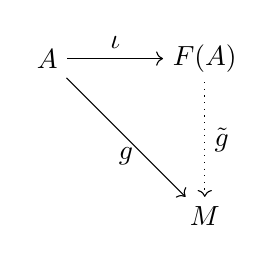
\begin{tikzpicture}
    \node (A) at (0,0) {$A$};
    \node (F) at (2,0) {$F(A)$};
    \node (M) at (2,-2) {$M$};
    \draw[->] (A)--(F) node[midway, above] {$\iota$};
    \draw[->] (A)--(M) node[midway, below] {$g$};
    \draw[dotted, ->] (F)--(M) node[midway, right] {$\tilde{g}$};
  \end{tikzpicture}
\exercise{Decode what this means!}
\item[Decomposition] We're often interested in decomposing modules
  into their smallest pieces... whatever that means. Here we define
  that. 
\item[Definition] If $M$ and $N$ are two $R$-modules, we define
  $M\oplus N$ to be the \emph{external direct sum}. That is, the set $\{(m,n)
  \mid m\in M, n\in N\}$ with addition and $R$-action defined
  componentwise. 
\item[Exercise] \exercise{Show that if $M$ and $N$ are both finitely
    generated, then so is $M\oplus N$. }
\item[Internal decomposition] We next want to ask whether a module $M$
  has submodules $N$ and $L$ so that $M$ is isomorphic to $N \oplus
  L$. Naturally, if $(n,l)\in N\oplus L$, we could probably define an
  element $\varphi(n,l)\in M$ via $n+l$. If we want this to be an
  isomorphism, $\varphi$ should be one-to-one and onto. 
\item[Definition] \exercise{Write the appropriate definition of an
    \emph{internal direct sum}. That is, if $M$ is an $R$-module with
    submodules $N, L$, then $N\oplus L \cong M$ if...}
\item[Exercise] \exercise{Consider the ring $R=\bbZ$, and $\bbZ$ as a
    module over itself. Prove that $\bbZ$ is \emph{not} a direct sum
    of any of its submodules.}
\item[Definition] An $R$-module $M$ is called \emph{decomposable} if
  $M\cong N\oplus L$ for some non-trivial $R$ modules $N, L$. It is
  called \emph{indecomposable} otherwise. (The definition can be
  written in a way similar to that of simple modules: $M$ is
  \emph{indecomposable} if $M\cong N\oplus L$ implies that $N=0$ or
  $N=M$.)
\item[Exercise] \exercise{Which of the $\bbZ$-modules of the form
    $\bbZ/n\bbZ$ are indecomposable?} 
\item[Direct sum decomposition] So \emph{when} is it the case that a
  module decomposes? We have something similar to the story for rings
  themselves. 
\item[Proposition] Let $N_1, \dotsc, N_k$ be submodules of the
  $R$-module $M$. The following are equivalent:
  \begin{itemize}
  \item The map $\pi: N_1\oplus \dotsc \oplus N_k \rightarrow
    N_1+N_2+\dotsc+N_k$ defined by 
    \[\pi(a_1,a_2,\dotsc, a_k) = a_1+a_2+\dotsc + a_k\] is an
    isomorphism of $R$-modules.
  \item $N_j\cap (N_1+N_2+\dotsc + \hat{N_j}+\dotsc + N_k) = 0$ for
    all $j$.
  \item Every $x\in N_1+\dotsc + N_k$ can be written uniquely in the
    form $a_1+a_2+\dotsc + a_k$ with $a_i \in N_i$. 
  \end{itemize}
\item[Example] Consider the $\bbC[t]$-module corresponding to the pair
  $M=\left(\bbC^2, \begin{bmatrix} 2&0  \\ 0 &
      3 \end{bmatrix}\right)$. Let $N_i$ be the subset
  $\operatorname{span}(e_i)$ (check that it's a submodule). Note that
  indeed $N_1\cap N_2=0$. So $M\cong N_1 \oplus N_2$. Now notice that
  $N_1$ is isomorphic to $(\bbC^1, [2])$ and $N_2$ is isomorphic to
  $(\bbC^1, [3])$. Note that these are both indecomposable $\bbC[t]$ modules.
\item[Example] The module $\bbZ/6\bbZ$  has $\bbZ$ submodules
  $N_1=\{0,2,4\}$ and $N_2=\{0,3\}$. Note that $N_1\cap N_2 =\{0\}$,
  so $N_1\oplus N_2 \cong N_1 + N_2$, and $N_1+N_2=\bbZ/6\bbZ$, so
  $\bbZ/6\bbZ\cong \bbZ/3\bbZ \oplus \bbZ/2\bbZ$. Note that these are
  both indecomposable $\bbZ$ modules, so we cannot further ``factor''
  this.
\item[Exercise] \exercise{Suppose that $M$ and $N$ can be generated by
    $m$ and $n$-element subsets, respectively. Prove that $M\oplus N$
    is can be generated by $m+n$ elements.}
\item[Exercise] \exercise{Suppose that $M$ is a finitely
    generated $R$-module. Prove that $M/L$ is finitely generated.}
\item[Exercise] \exercise{Suppose that $L$ and $M/L$ are finitely
    generated. Then $M$ is finitely generated. } This exercise forms a
  jumping-off point for us, in a way. We will often try to under stand
  modules by understanding their sub- and quotient modules. 
\item[Exercise] \exercise{Suppose that $M$ is an $R$-module, $M\neq
    0$. Prove that $M$ is irreducible if and only if $M$ is cyclic and
    can be generated by any of its non-zero elements. }
\item[Exercise] \exercise{Suppose that $R$ is commutative. Show that
    $M$ is irreducible if and only if $M\cong R/I$.}
\end{description}

\subsection{Tensor products of modules}
\label{sec:tens-prod-modul-1}

Let's work on a few analogies between vector spaces and modules: 

\begin{tabular}[h]{|l|l|}
  \hline
  Vector space over $F$ & Modules over $R$ \\ \hline \hline
  linear transformation & module homomorphism\\\hline
  vector subspace & submodule\\\hline
  quotient space & quotient module\\\hline
  dimension  & rank (of a free module) \\\hline
  direct sums of vector spaces & direct sums of modules\\\hline
  \begin{minipage}{0.4\linewidth}dimension of direct sum is sum of dimensions\end{minipage} & \begin{minipage}{0.4\linewidth}rank of the direct
                                                 sum is sum of the
                                                 ranks\end{minipage}\\\hline
  tensor product of vector spaces & tensor products of modules\\\hline
  \begin{minipage}{0.4\linewidth}dimension of tensor product is product of dimensions \end{minipage}& \begin{minipage}{0.4\linewidth}rank of
                                                         tensor
                                                         product is
                                                         tensor
                                                         product of
                                                         ranks\end{minipage}\\
\hline
\end{tabular}

Here's a ``categorification'' way to think about tensor products: 
\begin{itemize}
\item Zero dimensional vector spaces exist, it's just the singleton 0
  vector.
\item There is a vector space of dimension equal to each positive
  integer $n$, $F^n$. 
\item Given a vector space $V$ and a subspace $W$, we can construct a
  vector space of dimension $\dim V - \dim W$.
\item Given two vector spaces $V$ and $W$, we can construct a vector
  space of dimension $\dim V + \dim W$
\item What about a vector space of dimension $\dim V \cdot \dim W$?
\end{itemize}
\begin{description}
\item[Idea] Suppose that $V$ and $W$ are vector spaces over $F$ with
  bases $\{e_i\}$ and $\{f_j\}$. Build a new space $V\otimes_F W$ as
  the free vector space with basis $\{e_i \otimes f_j\mid i\in I, j\in
  J\}$. Then, for any $v\in V, w\in W$, define $v\otimes w$ to be the
  linear combination $\sum_{i,j} c_{ij}e_i\otimes f_j$ where
  $c_{ij}=[v]_i \cdot [w]_j$ (the entries of the column vector of $v$
  and $w$ written in their corresponding bases). 
\item[Example] $\bbR^2 \otimes_\bbR \bbR^3$ is 6D. We can show that
  the expression of an element is \emph{independent of basis chosen.}
  So $v\otimes w$ means something that has nothing to do with
  \emph{how} $v$ and $w$ are represented\footnote{Contrast with the
    dot product of two vectors, which is highly basis dependent.} 
\item[Notes] We \emph{should} be able to do the same thing for a
  module... but it's not clear how unless we have a basis...
\item[Notes] It does seem that we want some conditions to hold:
  linearity in the \emph{first} component and \emph{second} component
  separately.
\item[Definition] Let $M$ and $N$ be $R$ modules. A \emph{bilinear
    map} $B: M\times N \rightarrow P$ is a function which is linear in
  each component. Note that $B(-,n)$ and $B(m,-)$ are linear
  (homomorphisms) for each $m\in M$, $n\in N$. 
\item[Examples]
  \begin{enumerate}
  \item $B(v,w) = v\cdot w$ where $v,w\in \bbR^n$ is bilinear;
  \item Matrix multiplication $B(X,Y) = XY$ is bilinear from
    $\Mat_{m\times n}(R) \times \Mat_{n\times l}(R)$ whenever $R$ is
    commutative. 
  \item The cross-product is bilinear
  \item The determinant is multilinear: $\det: \underbrace{F^n \times F^n \times
    \dotsc \times F^n}_n \rightarrow F$
\item the module action $B: R\times M \rightarrow M$ is bilinear
\item Multiplication $R\times R \rightarrow R$ is bilinear
\item If $M^\vee=\Hom_R(M,R)$, then the \emph{dual pairing}
  $(\varphi, m) \mapsto \varphi(m)$ is bilinear
\item If $\varphi \in M^\vee, \psi \in N^\vee$, then the function
  $M\times N \rightarrow R$ given by $\varphi(m)\psi(n)$ is bilinear
\item If $M\times N\rightarrow P$ is bilinear, and $P\rightarrow Q$ is
  linear, then the composition is bilinear. 
\item \emph{We would like the function} $M\times N \rightarrow
  M\otimes_R N$ with $(m,n)\mapsto m\otimes n$ to be bilinear. 
  \end{enumerate}
\item[Note] Kernel is not a submodule (don't even know what the module
  structure on $M\times N$ is (but it's definitely not the normal one)
  and the image is not necessarily a submodule. 
\item[Important example] Consider the map $B: R^n \times R^n
  \rightarrow M_n(R)$ known as the \emph{outer product}. It gives
  $B(v,w) = vw^T$ where $v$ and $w$ are column vectors. Note that
  $B(e_1,e_1)+B(e_2,e_2) = I_2$ but the identity matrix is not equal
  to $B(v,w)$ for any vectors $v,w$ (since the outer product has rank
  1, as all columns are multiples of $v$). 
\item[Construction] Now that we have our wishlist: that (1) $M\otimes_R N$
  should be a module, (2) it should admit a bilinear map from $M\times
  N$ to itself and (3) should be ``as small as possible''. Hence, we
  get the universal property
    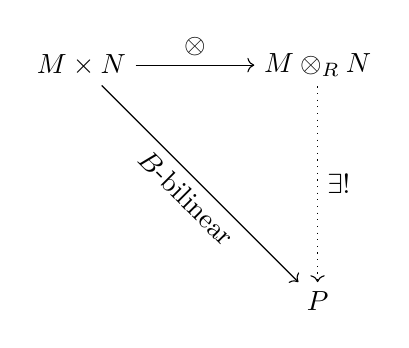
\begin{tikzpicture}
      \node (mxn) at (0,0) {$M\times N$};
      \node (motn) at (3,0) {$M\otimes_R N$};
      \node (p) at (3,-3) {$P$};
      \draw[->] (mxn)--(p) node[midway, below,rotate=-45] {$B$-bilinear};
      \draw[->] (mxn)--(motn) node[midway,above] {$\otimes$};
      \draw[dotted,->] (motn)--(p) node[midway,right] {$\exists !$};
    \end{tikzpicture}
  \item[Proposition] The tensor product, if it exists, is unique
    because of the universal property. 
  \item[Proposition] The tensor product exists.
    \begin{proof}
      Let $F_R(M\times N)$ be the MASSIVE free module with basis
      $e_{m,n}$ for every pair $(m,n)\in M\times N$. This is not just
      the set of ordered pairs: it is the set with a basis element for
      each ordered pair. It has \emph{rank} equal to $\lvert M\times
      N\rvert$.
      [Example:]
        If $M=\bbZ/2\bbZ$ and $N=\bbZ/3\bbZ$, then the corresponding
        $\bbZ$ module $F(M\times N)$ has rank $6$. Its elements look
        like \[a_{00} ([0],[0])+a_{10}(1,0) + a_{01}(0,1)+a_{11}(1,1)+a_{02}(0,2)+a_{12}(1,2).\]
      
We take $I$ to be the submodule of $F(M\times N)$ spanned by the
elements of the form:
\begin{align*}
  e_{m+m',n}-e_{m,n}-e_{m',n} \\
  e_{m,n+n'}-e_{m,n}-e_{m,n'}\\
e_{\lambda m, n} - \lambda e_{m,n}\\
e_{m,\lambda n}-\lambda e_{m,n}.
\end{align*}
Then $M\otimes_R N = F(M\times N)/I$. 
    \end{proof}
  \item[Remark] It's instructive to consider the difference between
    $M\oplus N$ and $M\otimes N$. For example, consider $R[x]\oplus
    R[y]$. This is the set of ordered pairs $(f(x), g(y))$ where $f$
    is a polynomial in $x$, and $g$ is a polynomial in $y$. We further
    consider them as sums, so that
    $(f(x),g(y))=(f(x),0)+(0,g(y))$. However, $R[x]\otimes R[y]$ has
    elements which are \emph{linear combinations} of pairs of
    polynomials. For example, \[\sum_{i,j} c_{ij}x^i y^j\in
      R[x]\otimes R[y],\] so $R[x]\otimes R[y]$ can be identified with
    $R[x,y]$. 
  \item[Example] $\bbQ\otimes_\bbZ \bbZ/n\bbZ=0$. Indeed, $(r\otimes
    k) = (r/n)n \otimes [k] = r/n \otimes [nk]=r/n\otimes 0 = 0.$
\item[Example] What does it mean if $m\otimes n=0$? It means that
  \emph{every} bilinear map from $M\times N$ to any module $P$ has
  $B(m,n)=0$. 
\item[Example] What does it mean if $M\otimes N=0$? It means that
  every bilinear map from $M\times N$ to any other module is the zero
  map. 
\item[Example] $\bbZ/n\bbZ \otimes_\bbZ \bbZ/m\bbZ\cong \bbZ/\gcd(n,m)\bbZ$
  \begin{proof}
    Suppose we have an element \[\sum_{i} a_i \otimes b_i.\] Then by
    using linearity, this is $(\sum_i a_ib_i)(1\otimes 1)$, so
    $(1\otimes 1)$ spans the tensor product. Note that $n(1\otimes
    1)=n\otimes 1=0$ and similarly with $m$, so the order or
    $(1\otimes 1)$ divides $m$ and $n$. Hence, the cardinality of the
    tensor product is bounded by $\gcd(m,n)$. 
In the other direction, let's actually create a bilinear
map. $\bbZ/n\bbZ\times \bbZ/m\bbZ \rightarrow \bbZ/d\bbZ$ given by
$(a,b) \mapsto [ab]_d$. It can be show that this is bilinear, so there
is a unique map from the tensor product to $\bbZ/d\bbZ$. Further,
$f(a,1)=[a\cdot 1]_d$, so $f$ is onto. 
  \end{proof}
\item[Example] $R/I\otimes R/J \cong R/(I+J)$ (use the map
  $(x,y)\mapsto xy$. 
\item[Example] $\bbZ/n\bbZ \otimes_\bbZ A \cong A/n\bbZ$ for any
  abelian group $A$. 
\item[Example] $\Hom_R(M,N) \cong M^\vee \otimes N$ when $M$ is
  finitely-generated and free. (At least, think about the
  generalization). 
\item[Example] $R\otimes_R M \cong M$
\item[Example] $F\otimes_R F'$ is free when $F$ and $F'$ are (and the
  basis works nicely too). 
\item[Example] $F\otimes_R M$ has elements with unique representation
  as $\sum_{i\in I} m_i \otimes e_i$ where all but finitely many of
  the summands are zero. 
\item[Example] (Excellent example to know) Extension of scalars:
  Suppose that $S\subset R$ is a subring. Hence, every module over $R$
  is a module over $S$. But, we can go the other way around. $R$ is an
  $S$-module. Assume $M$ is also an $S$ module. Then $R\otimes_S M$ is
  now an $R$-module (since $R$ can act on the first component). 




\end{description}
\subsection{Exact sequences and special modules}
\label{sec:exact-sequ-spec-1}

Buoyed by a few of the theorems from the section on modules (where
understanding a submodule and quotient module can let us understand
the module itself. 

\begin{description}
\item[Sequence of morphisms] A \emph{sequence of morphisms}
  \[\rightarrow X_1\xrightarrow{f_1} X_2 \xrightarrow{f_2} X_3
    \xrightarrow{f_3} X_4\rightarrow \dotsc\] is \emph{exact at $X_n$}
    if $\ker f_n=\image f_{n-1}$. 
  \item[Example] As an example, $0\rightarrow X \xrightarrow{f} Y$ is
    exact at $X$ if and only if $\ker f=\image 0=0$, so if and only if
    $f$ is one-to-one. 
  \item[Example] Similarly, $Y\xrightarrow{g} Z \xrightarrow{h} 0$ is
    exact at $Z$ if and only if $Z=\ker h = \image g$, so if and only
    if $g$ is onto. 
  \item[Example] The sequence \[\bbZ/4\bbZ \xrightarrow{3\cdot n}
      \bbZ/6\bbZ \xrightarrow{\textrm{reduce mod 3}} \bbZ/3\bbZ\] is
    exact at $\bbZ/6\bbZ$. The kernel of reduction mod 3 is $\{0,3\}$,
    which is the image of the first morphism. 
  \item[Definition] A sequence \[0 \rightarrow X \xrightarrow{\varphi}
      Y \xrightarrow{\psi} Z \rightarrow 0\] is called a \emph{short
      exact sequence} of it is exact at $X$, $Y$, and $Z$. 
  \item[Example] If we work with arbitrary groups, the sequence \[0
      \rightarrow \bbZ/3\bbZ \xrightarrow{\overline{1}\mapsto (123)}
      S_3 \xrightarrow{sgn} \bbZ/2\bbZ \rightarrow 0.\]
  \item[Example] \[0 \rightarrow X \rightarrow X\oplus Z \rightarrow
      Z\rightarrow 0\]
  \item[Example] Here's one that may look interesting: 
\[0 \rightarrow \bbZ \xrightarrow{n\cdot } \bbZ \xrightarrow{[-]_n}
  \bbZ/n\bbZ \rightarrow 0\] It seems like the middle should be
``bigger'' than the outer pieces, but that's not true. 
\item[Example] Also, end terms don't uniquely determine the inner
  term: 
  \begin{align*}
    0 \rightarrow \langle r^2 \rangle \rightarrow D_4 \rightarrow
    D_4/\langle r^2\rangle \rightarrow 0 \\
 0 \rightarrow \{\pm 1\} \rightarrow Q_8 \rightarrow
    Q_8/ \{\pm 1\} \rightarrow 0 
  \end{align*}
\item[Example] There's a canonical short exact sequence associated
  with any homomorphism $f: M\rightarrow N$, namely: \[0 \rightarrow
    \ker f \rightarrow N \rightarrow \operatorname{image}(f)
    \rightarrow 0 \]
\item[Example] Let $M$ be a finitely-generated $R$-module, generated by
  $\{m_1,m_2,\dotsc, m_t\}$. Let $R^t$ be the free $R$-module of rank
  $t$. Then we have the homomorphism $\varphi: R^t \rightarrow M$ with
  $\varphi(e_i) = m_i$, which is onto. The \emph{kernel} is referred
  to as the module of relations: \[0 \rightarrow K \rightarrow R^t
    \rightarrow M \rightarrow 0.\]
\item[Specific example] Consider the ring $R=\bbC[x,y]$, and the ideal
  $I=(x,y).$ There is an onto map from $R^2$ to $I$ sending $e_1$ to
  $x$ and $e_2$ to $y$. Notice that
  \begin{align*}
    \ker \pi &= \{fe_1+ge_2 \mid \pi(fe_1+ge_2)=0\}\\
    &= \{fe_1+ge_2 \mid fx+gy=0\}\\
    &= \{fe_1+ge_2 \mid fx=-gy\}\\
    &= \{\chi (y,-x) \mid \chi \in R\}.
  \end{align*}
Then we have the exact sequence: 
  \[0 \rightarrow R\xrightarrow{e_1 \mapsto (y,-x)} R^2
    \xrightarrow{\begin{matrix} e_1 \mapsto x\\ e_2 \mapsto y\end{matrix}} I\rightarrow 0.\]
\item[Example] $R=\bbC[t]$, $M=\bbC$ the module with $t.a=0$, and $N$
  the module $\bbC^2$ with $t.e_1=0$ and
  $t.e_2=e_1$. Then \[0\rightarrow M \xrightarrow{\begin{bmatrix} 0\\1\end{bmatrix}} N
    \xrightarrow{\begin{bmatrix} 1\ 0\end{bmatrix} } M \rightarrow 0\]
\item[Example] A type $A_2$ example. In particular, \[0\rightarrow (0,\bbC,0)
    \rightarrow (\bbC,\bbC,1)\rightarrow (\bbC, 0, 0)\rightarrow 0\]
\item[Splitting] A short exact sequence is called \emph{split} if
  $Y\cong X\oplus Z$. 
\item[Criterion for splitting: sections and retractions] Suppose that 
  \[\eta=0 \rightarrow X \xrightarrow{f} Y \xrightarrow{g} Z \rightarrow
    0 \] is a short exact sequence, and that there exists a
  homomorphism $g': Z\rightarrow Y$ such that $g\circ g' = id_Z$. Then
  $\eta$ is a split exact sequence.
  \begin{proof}
    Given the above conditions, consider the submodules $x=\image(f)$ and $z=\image(g')$ in
    $Y$. Since $f$ and $g'$ are injective, $X\cong x$ and $z\cong
    Z$. Furthermore, $x\cap z = \{y\in Y \mid y=f(x)=g'(z)\}$, but if
    this is the case, then
    \begin{align*}
      g(f(x)) &= g(g'(z))\\
      0 &= z
    \end{align*}
so $z=0$, hence, $x=0$ and $y=0$. Thus, $x\cap z=0$. Furthermore, if
$y\in Y$, we claim $y=x+z$ for some $x\in f(X)$, and $z\in
g'(Z)$. Indeed, let  $z=g'\circ g(y)\in Z$. Then $g(z-y) =
gg'g(z)-g(y) = g(y)-g(y)=0$, so $z-y=x$ for some $x\in F(X)$. Hence,
$y=z-x$. Thus, $X\oplus Z \cong f(X)+g'(Z)\cong Y$. 
  \end{proof}
\item[Retractions] Dually, a retraction is a homomorphism
  $f':Y\rightarrow X$ such that $f'\circ f=id_X$. The dual proposition
  is that if there exists a retraction, then $\eta$ splits. 
\item[Example] If \[\eta=0 \rightarrow X \xrightarrow{f} Y \xrightarrow{g} Z \rightarrow
    0 \] is a short exact sequence with $Z$ free, then $\eta$ splits.
  \begin{proof}
    By the discussion on sections, we can simply show that there
    exists a section. Suppose that $Z$ is free with basis $\{z_\alpha
    \mid \alpha \in A\}$. Then, since $g$ is a surjection, there exist
    elements $y_\alpha \in Y$ such that $g(y_\alpha)=z_\alpha$ for
    each $\alpha$. Define the map $g'$ with
    $g'(z_\alpha)=y_\alpha$. From the universal property of free
    modules, this extends to a homomorphism, and clearly
    $gg'(z_\alpha)=g(y_\alpha)=z_\alpha$ for each $\alpha$. 
  \end{proof}
So what this says is that any short exact sequence with free right end
splits. Are there other modules with this property? 


 
\item[Definition] An $R$-module $P$ is called \emph{projective} if
  every short exact sequence \[0 \rightarrow X \rightarrow Y
    \rightarrow P \rightarrow 0 \] splits. (Equivalently, every onto
  map $Y\rightarrow P$ has a section.)
\item[Example] Free modules are projective (see corollary above)
\item[Example] Consider the ring $R=\bbC[t]/(t^n)$. Then the only indecomposable
  (finite-dimensional) non-zero projective $R$-module is itself. 
\item[Example] Consider the path algebra of $1\rightarrow 2$. Its
  indecomposable projective modules are $F \xrightarrow{[1]} F$ and
  $0\xrightarrow{} F$. 
\item[Convenience] It's convenient to think about the $\Hom(-,-)$
  functor. 
\item[Proposition] TFAE for an $R$-module $P$
  \begin{enumerate}
  \item $P$ is projective
  \item There exists a module $Q$ such that $P\oplus Q$ is free.
    \item If $\pi: M\rightarrow N$ is surjective and $\varphi:
      P\rightarrow N$ is a homomorphism, then there exists a
      homomorphism $\Phi: P\rightarrow M$ such that $\varphi= \pi
      \circ \Phi$
    \item If $\pi: M\rightarrow N$ is a surjection, the natural map
      $\Hom(P, M) \rightarrow \Hom(P,N)$ is surjective. 
  \end{enumerate}
\item[Definition] $\Hom_R(P,-)$ is a \emph{functor} from $\mod(R)$ to
  $\Ab$. That is, an assignment of an abelian group $\Hom_R(P,M)$ to
  each module $M$ in $\mod(R)$ and a morphism $\Hom_R(P,f):
  \Hom_R(P,M)\rightarrow \Hom_R(P,N)$ for each
  morphism $f: M\rightarrow N$. (This is called \emph{covariant}.)
\item[Proposition] $\Hom_R(P,-)$ is \emph{left-exact}, meaning that if
  $f:M\rightarrow N$ is injective, so is $\Hom_R(P,f)$. It is not
  necessarily right-exact. Indeed, consider $M=\bbZ/4\bbZ$,
  $N=\bbZ/2\bbZ$ and the projection, and $P=\bbZ/2\bbZ$. Then
  $\Hom_R(P,M)=\{[2x]_4, [0]_0\}$ and $\Hom_R(P,N)= \{[x]_2,
  [0]_2\}$. However, $f=[x]_2$, so any composition of it with
  something in $\Hom_R(P,M)$ is zero.
  \begin{proof}
    Suppose that $f:M\rightarrow N$ is injective. We have the map
    $\Hom_R(P,M)\xrightarrow{f\circ -} \Hom_R(P,N)$ defined by
    composition, so suppose $f\circ \varphi_1 = f\circ \varphi_2$ for
    some morphisms $\varphi_i \in \Hom_R(P,M)$. Then
    $f(\varphi_1(x))=f(\varphi_2(x))$ for all $x\in P$. But $f$ is
    injective, so $\varphi_1(x)=\varphi_2(x)$ for all $x\in P$. Hence,
    $\varphi_1=\varphi_2$. 
  \end{proof}


\end{description}

\section{Algebraic geometry}
\label{sec:algebraic-geometry-1}

The origins of algebraic geometry lie in the solutions to systems of
polynomial equations. You've already seen a subset of this topic in
linear algebra, which originates as the study of the solutions to
systems of linear equations. The ``geometric'' part there was that
solutions to systems of linear equations were (affine) vector spaces,
which could be obtained by finding one particular solution and the
family of homogeneous solutions. We then showed that every solution is
a sum of your particular solution and a homogeneous solution. We
further saw what happened if we wanted to ``intersect'' these spaces:
you get another (affine) vector space, and the dimension of the
intersection can be understood as bounded by certain dimensions.

Now suppose that we have a system of polynomial equations:
\begin{align*}
  a^2+b^2+c^2+d^2&=1\\
                  ab+cd&=0\\
                   ac+bd&=0\\
  ad+bc&=0.
\end{align*}

(This actually came up on a homework problem.) You'll quickly find
there are subcases based on whether one element is 0 or not and how
they relate to the others. It is, generally, a pain. 

\begin{description}
\item[Reframing] Let $R=\bbQ[x_1,\dotsc, x_n]$ be the polynomial ring
  in $n$ variables. Let $F=\{f_1,\dotsc, f_m\} \subset R$ be a collection of
  polynomials. We seek to compute (or at least understand in some way) 
  \[V(F) := \{(a_1,\dotsc, a_n) \mid f_i(a_1,\dotsc, a_n)=0 \forall
    i\}\] called the \emph{vanishing set of $F$}. 
\item[Example] Let $F=\{x^2+y^2+z^2-1, x+y+z\}$, then $V(F)$ is the
  cross-section of the sphere of radius $1$ with the plane
  $x+y+z=0$. What does this look like? 
\item[Note] Suppose that $\underline{a}$ is a solution to each
  $f_i$. Then it is also a solution to 
  \[\sum c_i f_i\] for all choices of functions $c_i \in R$. In
  particular, this shows that $V(F) = V( RF)$ where $RF$ is the ideal
  generated by $F$. 
\item[Definition] A set $Z\in \bbA^n$ is called \emph{algebraic} if
  $Z=V(J)$ for some ideal $J\subset R$.  
\item[Other direction] Now given a set of points $Z\subset \bbA^n$, we
  could ask ``which functions vanish at all of them?'' This is called
  the \emph{ideal} of $Z$, denoted $I(Z)$. 
\item[Example] $I(\{(1,1)\}) = (x-1,y-1)$
\item[Bouncing] What happens when we bounce back-and-forth? Well,
  $V(I(Z))$ is not necessarily equal to $Z$, but it certainly contains
  $Z$. It is exactly $Z$ precisely when $Z$ is an algebraic set. Furthermore, $I(V(J))$ is not necessarily $J$, but it contains
  $J$. The reason that $I(V(J))\neq J$ is given by the following
  example.
\item[Example] $J=(x^2-2xy+y^2)$. $V(J) = \{(a,b) \mid
  a^2-2ab+b^2=0\}$ but this is the same as saying $(a-b)^2=0$, so
  $a=b$. Thus, $V(J) = \{(a,a) \mid a\in F\}$. It's not hard to show
  that $I(V(J))=(x-y)$. You see, $f=(x-y)^2$, so $f(a,b)=0$ if and
  only if $(x-y)=0$. 
\item[Definition] An ideal $J\subset R$ is called \emph{radical} if
  $f^n \in I$ for some $n>0$ implies $f\in J$. So $J$ is closed under
  taking $n$-th roots for any $n$. 
\item[Theorem: Hilbert Nullstellensatz] $I(V(J))=\sqrt{J}$, where
  $\sqrt{J}$ is the set $\{r\in R \mid r^n \in J \exists n>0\}$. 
\item[What?] So really, the study of algebraic sets is equivalent to
  the study of radical ideals. Sets $X$ such that $X=V(J)$ for $J$ a
  radical ideal are called \emph{algebraic varieties}. 
\item[Algebra/Geometry] Here's a question: when can you break your set
  into pieces?
\item[Definition] $Z$ is called \emph{irreducible} if $Z=Z_1\cup Z_2$
  implies $Z=Z_1$ or $Z=Z_2$. (Hence, $Z$ cannot be written as a union
  of strictly smaller varieties. )
\item[Theorem]   The variety $V$ is irreducible if and only if $I(V)$
  is prime.
  \begin{proof}
    If $V$ is irreducible, let $I(V)$ be its ideal. If $fg\in I$ but
    $f,g\notin I$, then define $V_1=V(I+\langle f\rangle)\subsetneq
    V(I)$ and $V_2=V(I+\langle g\rangle)\subsetneq V(I)$. But $x\in V$
    is either in $V_1$ or $V_2$, so $V=V_1\cup V_2$. 
On the other hand, if $I$ is prime, and $V(I)$ is reducible, then
$V=V_1\cup V_2$ with $V_i\subsetneq V$. So we can find $f\in
I(V_1)\setminus I(V_2)$ and $g\in I(V_2)\setminus I(V_1)$. Note $fg\in
I$ since $fg$ kills anything in $V_1$ or $V_2$; but $I$ is prime. 
  \end{proof}
\item[Dimension] So now let's think about dimension. Things are
  different in algebraic geometry than Euclidean. In particular,
  suppose that we have irreducible varieties such that $Z_1\supsetneq
  Z_2 \supsetneq \dotsc$. This means that we have a sequence of prime
  ideals $I(Z_1)\subsetneq I(Z_2) \subsetneq \dotsc$ all in
  $R$. However, the famous ``Hilbert Basis Theorem'' says that
  $\bbC[x_1,\dotsc, x_n]$ is a so-called \emph{Noetherian ring}, which
  means that the ideals stabilize. Hence, there are no infinitely
  descending chains of irreducible subvarieties of $\bbA^n$ (compare
  to the scenario with balls of radius $r$ for any $r$). Furthermore,
  the analytic dimension (Euclidean) of $Z_i$ is decreasing (again,
  compare to the Euclidean case). 
\item[Example] In $\bbC[x,y]$, we have the unit circle $C=\{(a,b) \mid
  a^2+b^2-1=0\}$. I.e., $C=V(x^2+y^2-1)$. The ideal generated by
  $x^2+y^2-1$ is prime. If we intersect this set with $x=0$ and take
  one of the two pieces, we have $V(x,y-1)$, which is a point, and
  $(x,y-1)$ is a maximal ideal, so there are no larger ideals other
  than $R$. So we have: $circ\supset point \supset \emptyset$ given by
  $(x^2+y^2-1)\subset (x,y-1) \subset R$. 
\end{description}


\section{Multilinear algebra}
\label{sec:multilinear-algebra}

Let's think about the way the determinant works: it is a function on
the columns (let's say) of a matrix, which returns an element of the
ground field. If $\dim V=n$ then \[\det:
  \underbrace{V\times V\times\dotsc \times V}_n
  \rightarrow F\] is the map defined by \[\det(v_1,\dotsc, v_n) =
  \det \begin{bmatrix} | & | & \dotsc & | \\ v_1 & v_2 & \dotsc &
    v_2\\| & | & \dotsc & |\end{bmatrix}.\] We've already seen that
it's multilinear, so really it is a homomorphism from $V^{\otimes n}$
to $F$. (If we want to be really fancy, $\Hom_F(V^{\otimes n}, F)
\cong (V^{\otimes n})^* \otimes_F F \cong (V^*)^{\otimes n}$, so the
determinant is nothing but an element of this big tensor product. 

But more than that, we have an extra relation held by the
determinant. Namely $\det (v_{(1,2,\dotsc,v_n)}) =(-1)^{\operatorname{sign}
  \sigma}\det(v_{\sigma(1,2,\dotsc, n)})$. It is a so-called
\emph{alternating} function (this is equivalent to the fact that if
two of the vectors are equal, the element is equal. We have another
relationship: alternating, let's make a universal property. 
\begin{description}
\item[Definition] Let $V$ be a free $F$-module, and $k$ an
  integer. $\bigwedge^k V$, the $k$-th exterior power of $V$, is the
  module with the following properties:
\begin{itemize}
\item There is a multilinear, alternating map $\wedge:
  \underbrace{V\times \dotsc \times V}_k\rightarrow \bigwedge^k V$ and
\item  For any multilinear, alternating
  function $M: \underbrace{V\times \dotsc \times V}_k \rightarrow P$,
  there is a unique homomorphism $\Psi: \bigwedge^k V \rightarrow P$
  such that $\Psi\circ \wedge = M$. 
\end{itemize}
\item[Remark]  The construction of $\bigwedge^k V$ is easy once you
  have the tensor product: simply take $V^{\otimes k}/I$ where $I$ is
  the ideal generated by all sums of the form $v_1 \otimes \dotsc
  \otimes v_k + v_{\sigma(1)} \otimes \dotsc \otimes
  v_{\sigma(k)}$. The equivalence class of $v_1\otimes \dotsc \otimes
  v_k$ in $\bigwedge^k V$ is denoted $v_1 \wedge \dotsc \wedge v_k$. 
\item[Example] Consider the element $(5e_1+2e_2) \wedge (e_1 + 3e_2)$
  in $\bigwedge^2(F^2)$. Using the relations, we have
  \begin{align*}
    (5e_1+2e_2) \wedge (e_1 + 3e_2) &= 5\cdot 1 e_1 \wedge e_1 +
                                      2\cdot 1 e_2 \wedge e_1 \\
& \qquad 5 \cdot 3 e_1 \wedge e_2 + 2\cdot 3 e_2 \wedge e_2\\
  &= (5\cdot 3 - 2 \cdot 1 ) e_1 \wedge e_2.
  \end{align*}
Look familiar? Indeed, we can consider the determinant function $\det:
F^2 \times F^2 \rightarrow F$. Because of the universal property,
there is a unique function $\Psi: \bigwedge^2(F^2) \rightarrow F$ with
$\Psi(v\wedge w) = \det(v,w)$. It's clearly the function which takes
$v\wedge w$ to $\det(v,w)$.
\item[Example] Consider the function $M: \bbR^3 \times
  \bbR^3\rightarrow \bbR^3$
  given by the following: $M(v, w) = \langle v_2w_3-v_3w_2,
  -(v_1w_3-v_3w_1),v_1w_2-v_2w_1\rangle$. (Note that $M$ is the usual
  cross-product from multivariable calculus.) This gives us a linear
  function $\Psi: \bigwedge^2(\bbR^3)\rightarrow \bbR^3$ with
  $\Psi(v\wedge w) = v\times w$. This is used heavily in differential
  geometry. 
\item[Utility] 
\end{description}
\end{document}
2018/01/02 02:54:54
